% Options for packages loaded elsewhere
\PassOptionsToPackage{unicode}{hyperref}
\PassOptionsToPackage{hyphens}{url}
%
\documentclass[
]{article}
\usepackage{amsmath,amssymb}
\usepackage{lmodern}
\usepackage{iftex}
\ifPDFTeX
  \usepackage[T1]{fontenc}
  \usepackage[utf8]{inputenc}
  \usepackage{textcomp} % provide euro and other symbols
\else % if luatex or xetex
  \usepackage{unicode-math}
  \defaultfontfeatures{Scale=MatchLowercase}
  \defaultfontfeatures[\rmfamily]{Ligatures=TeX,Scale=1}
\fi
% Use upquote if available, for straight quotes in verbatim environments
\IfFileExists{upquote.sty}{\usepackage{upquote}}{}
\IfFileExists{microtype.sty}{% use microtype if available
  \usepackage[]{microtype}
  \UseMicrotypeSet[protrusion]{basicmath} % disable protrusion for tt fonts
}{}
\makeatletter
\@ifundefined{KOMAClassName}{% if non-KOMA class
  \IfFileExists{parskip.sty}{%
    \usepackage{parskip}
  }{% else
    \setlength{\parindent}{0pt}
    \setlength{\parskip}{6pt plus 2pt minus 1pt}}
}{% if KOMA class
  \KOMAoptions{parskip=half}}
\makeatother
\usepackage{xcolor}
\usepackage[margin=1in]{geometry}
\usepackage{color}
\usepackage{fancyvrb}
\newcommand{\VerbBar}{|}
\newcommand{\VERB}{\Verb[commandchars=\\\{\}]}
\DefineVerbatimEnvironment{Highlighting}{Verbatim}{commandchars=\\\{\}}
% Add ',fontsize=\small' for more characters per line
\usepackage{framed}
\definecolor{shadecolor}{RGB}{248,248,248}
\newenvironment{Shaded}{\begin{snugshade}}{\end{snugshade}}
\newcommand{\AlertTok}[1]{\textcolor[rgb]{0.94,0.16,0.16}{#1}}
\newcommand{\AnnotationTok}[1]{\textcolor[rgb]{0.56,0.35,0.01}{\textbf{\textit{#1}}}}
\newcommand{\AttributeTok}[1]{\textcolor[rgb]{0.77,0.63,0.00}{#1}}
\newcommand{\BaseNTok}[1]{\textcolor[rgb]{0.00,0.00,0.81}{#1}}
\newcommand{\BuiltInTok}[1]{#1}
\newcommand{\CharTok}[1]{\textcolor[rgb]{0.31,0.60,0.02}{#1}}
\newcommand{\CommentTok}[1]{\textcolor[rgb]{0.56,0.35,0.01}{\textit{#1}}}
\newcommand{\CommentVarTok}[1]{\textcolor[rgb]{0.56,0.35,0.01}{\textbf{\textit{#1}}}}
\newcommand{\ConstantTok}[1]{\textcolor[rgb]{0.00,0.00,0.00}{#1}}
\newcommand{\ControlFlowTok}[1]{\textcolor[rgb]{0.13,0.29,0.53}{\textbf{#1}}}
\newcommand{\DataTypeTok}[1]{\textcolor[rgb]{0.13,0.29,0.53}{#1}}
\newcommand{\DecValTok}[1]{\textcolor[rgb]{0.00,0.00,0.81}{#1}}
\newcommand{\DocumentationTok}[1]{\textcolor[rgb]{0.56,0.35,0.01}{\textbf{\textit{#1}}}}
\newcommand{\ErrorTok}[1]{\textcolor[rgb]{0.64,0.00,0.00}{\textbf{#1}}}
\newcommand{\ExtensionTok}[1]{#1}
\newcommand{\FloatTok}[1]{\textcolor[rgb]{0.00,0.00,0.81}{#1}}
\newcommand{\FunctionTok}[1]{\textcolor[rgb]{0.00,0.00,0.00}{#1}}
\newcommand{\ImportTok}[1]{#1}
\newcommand{\InformationTok}[1]{\textcolor[rgb]{0.56,0.35,0.01}{\textbf{\textit{#1}}}}
\newcommand{\KeywordTok}[1]{\textcolor[rgb]{0.13,0.29,0.53}{\textbf{#1}}}
\newcommand{\NormalTok}[1]{#1}
\newcommand{\OperatorTok}[1]{\textcolor[rgb]{0.81,0.36,0.00}{\textbf{#1}}}
\newcommand{\OtherTok}[1]{\textcolor[rgb]{0.56,0.35,0.01}{#1}}
\newcommand{\PreprocessorTok}[1]{\textcolor[rgb]{0.56,0.35,0.01}{\textit{#1}}}
\newcommand{\RegionMarkerTok}[1]{#1}
\newcommand{\SpecialCharTok}[1]{\textcolor[rgb]{0.00,0.00,0.00}{#1}}
\newcommand{\SpecialStringTok}[1]{\textcolor[rgb]{0.31,0.60,0.02}{#1}}
\newcommand{\StringTok}[1]{\textcolor[rgb]{0.31,0.60,0.02}{#1}}
\newcommand{\VariableTok}[1]{\textcolor[rgb]{0.00,0.00,0.00}{#1}}
\newcommand{\VerbatimStringTok}[1]{\textcolor[rgb]{0.31,0.60,0.02}{#1}}
\newcommand{\WarningTok}[1]{\textcolor[rgb]{0.56,0.35,0.01}{\textbf{\textit{#1}}}}
\usepackage{graphicx}
\makeatletter
\def\maxwidth{\ifdim\Gin@nat@width>\linewidth\linewidth\else\Gin@nat@width\fi}
\def\maxheight{\ifdim\Gin@nat@height>\textheight\textheight\else\Gin@nat@height\fi}
\makeatother
% Scale images if necessary, so that they will not overflow the page
% margins by default, and it is still possible to overwrite the defaults
% using explicit options in \includegraphics[width, height, ...]{}
\setkeys{Gin}{width=\maxwidth,height=\maxheight,keepaspectratio}
% Set default figure placement to htbp
\makeatletter
\def\fps@figure{htbp}
\makeatother
\setlength{\emergencystretch}{3em} % prevent overfull lines
\providecommand{\tightlist}{%
  \setlength{\itemsep}{0pt}\setlength{\parskip}{0pt}}
\setcounter{secnumdepth}{-\maxdimen} % remove section numbering
\ifLuaTeX
  \usepackage{selnolig}  % disable illegal ligatures
\fi
\IfFileExists{bookmark.sty}{\usepackage{bookmark}}{\usepackage{hyperref}}
\IfFileExists{xurl.sty}{\usepackage{xurl}}{} % add URL line breaks if available
\urlstyle{same} % disable monospaced font for URLs
\hypersetup{
  pdftitle={MSGARCH-model strategy-test},
  hidelinks,
  pdfcreator={LaTeX via pandoc}}

\title{MSGARCH-model strategy-test}
\author{}
\date{\vspace{-2.5em}}

\begin{document}
\maketitle

\begin{Shaded}
\begin{Highlighting}[]
\FunctionTok{rm}\NormalTok{(}\AttributeTok{list =} \FunctionTok{ls}\NormalTok{())}
\FunctionTok{library}\NormalTok{(}\StringTok{"MSGARCH"}\NormalTok{)}
\FunctionTok{options}\NormalTok{(}\AttributeTok{prompt =} \StringTok{"R\textgreater{} "}\NormalTok{, }\AttributeTok{continue =} \StringTok{"+  "}\NormalTok{, }\AttributeTok{width =} \DecValTok{70}\NormalTok{,}
        \AttributeTok{digits =} \DecValTok{4}\NormalTok{, }\AttributeTok{max.print =} \DecValTok{80}\NormalTok{, }\AttributeTok{useFancyQuotes =} \ConstantTok{FALSE}\NormalTok{)}
\NormalTok{tmp }\OtherTok{\textless{}{-}} \FunctionTok{sessionInfo}\NormalTok{()}
\NormalTok{nam }\OtherTok{\textless{}{-}} \FunctionTok{paste0}\NormalTok{(}\StringTok{"PART\_II\_R"}\NormalTok{, tmp}\SpecialCharTok{$}\NormalTok{R.version}\SpecialCharTok{$}\NormalTok{major, }\StringTok{"."}\NormalTok{,}
\NormalTok{              tmp}\SpecialCharTok{$}\NormalTok{R.version}\SpecialCharTok{$}\NormalTok{minor, }\StringTok{"\_"}\NormalTok{, tmp}\SpecialCharTok{$}\NormalTok{R.version}\SpecialCharTok{$}\NormalTok{os)}
\FunctionTok{sink}\NormalTok{(}\AttributeTok{file =} \FunctionTok{paste0}\NormalTok{(}\StringTok{"sink\_"}\NormalTok{, nam, }\StringTok{".txt"}\NormalTok{), }\AttributeTok{append =} \ConstantTok{FALSE}\NormalTok{, }\AttributeTok{split =} \ConstantTok{TRUE}\NormalTok{) }\CommentTok{\# output printed in txt}
\FunctionTok{print}\NormalTok{(tmp)}
\end{Highlighting}
\end{Shaded}

\begin{verbatim}
## R version 4.2.2 (2022-10-31)
## Platform: aarch64-apple-darwin20 (64-bit)
## Running under: macOS Ventura 13.1
## 
## Matrix products: default
## BLAS:   /Library/Frameworks/R.framework/Versions/4.2-arm64/Resources/lib/libRblas.0.dylib
## LAPACK: /Library/Frameworks/R.framework/Versions/4.2-arm64/Resources/lib/libRlapack.dylib
## 
## locale:
## [1] en_US.UTF-8/en_US.UTF-8/en_US.UTF-8/C/en_US.UTF-8/en_US.UTF-8
## 
## attached base packages:
## [1] stats     graphics  grDevices utils     datasets  methods  
## [7] base     
## 
## other attached packages:
## [1] MSGARCH_2.51
## 
## loaded via a namespace (and not attached):
##  [1] Rcpp_1.0.9       rstudioapi_0.14  knitr_1.41      
##  [4] magrittr_2.0.3   fanplot_4.0.0    lattice_0.20-45 
##  [7] rlang_1.0.6      fastmap_1.1.0    stringr_1.5.0   
## [10] tools_4.2.2      grid_4.2.2       xfun_0.36       
## [13] cli_3.6.0        coda_0.19-4      htmltools_0.5.4 
## [16] yaml_2.3.6       digest_0.6.31    lifecycle_1.0.3 
## [19] Matrix_1.5-1     vctrs_0.5.1      codetools_0.2-18
## [22] glue_1.6.2       evaluate_0.19    rmarkdown_2.19  
## [25] stringi_1.7.12   compiler_4.2.2   expm_0.999-7    
## [28] zoo_1.8-11
\end{verbatim}

\hypertarget{load-smi}{%
\subsection{load SMI}\label{load-smi}}

\begin{Shaded}
\begin{Highlighting}[]
\FunctionTok{data}\NormalTok{(}\StringTok{"SMI"}\NormalTok{, }\AttributeTok{package =} \StringTok{"MSGARCH"}\NormalTok{)}

\DocumentationTok{\#\# Create MS(2){-}GJR{-}std specification (Ardia 2008 and Ardia et al. 2008)}
\NormalTok{ms2.gjr.s }\OtherTok{\textless{}{-}} \FunctionTok{CreateSpec}\NormalTok{(}\AttributeTok{variance.spec =} \FunctionTok{list}\NormalTok{(}\AttributeTok{model =} \StringTok{"gjrGARCH"}\NormalTok{),}
                        \AttributeTok{distribution.spec =} \FunctionTok{list}\NormalTok{(}\AttributeTok{distribution =} \StringTok{"std"}\NormalTok{),}
                        \AttributeTok{switch.spec =} \FunctionTok{list}\NormalTok{(}\AttributeTok{K =} \DecValTok{2}\NormalTok{),}
                        \AttributeTok{constraint.spec =} \FunctionTok{list}\NormalTok{(}\AttributeTok{regime.const =} \StringTok{"nu"}\NormalTok{))}

\DocumentationTok{\#\# ML estimation}
\NormalTok{fit.ml }\OtherTok{\textless{}{-}} \FunctionTok{FitML}\NormalTok{(ms2.gjr.s, }\AttributeTok{data =}\NormalTok{ SMI)}

\DocumentationTok{\#\# Summary}
\FunctionTok{summary}\NormalTok{(fit.ml)}
\end{Highlighting}
\end{Shaded}

\begin{verbatim}
## Specification type: Markov-switching
## Specification name: gjrGARCH_std gjrGARCH_std
## Number of parameters in each variance model: 4 4
## Number of parameters in each distribution: 1 1
## ------------------------------------------
## Fixed parameters:
## None
## ------------------------------------------
## Across regime constrained parameters:
## nu 
## ------------------------------------------
## Fitted parameters:
##          Estimate Std. Error  t value  Pr(>|t|)
## alpha0_1   0.2071     0.0488   4.2433 1.101e-05
## alpha1_1   0.0005     0.0088   0.0569 4.773e-01
## alpha2_1   0.2137     0.0619   3.4505 2.798e-04
## beta_1     0.5264     0.0995   5.2915 6.065e-08
## nu_1       9.2469     1.3292   6.9568 1.740e-12
## alpha0_2   0.0922     0.0349   2.6396 4.150e-03
## alpha1_2   0.0052     0.0169   0.3057 3.799e-01
## alpha2_2   0.1516     0.0381   3.9770 3.490e-05
## beta_2     0.8716     0.0354  24.6392    <1e-16
## P_1_1      0.9977     0.0014 701.8053    <1e-16
## P_2_1      0.0027     0.0017   1.6008 5.471e-02
## ------------------------------------------
## Transition matrix:
##       t+1|k=1 t+1|k=2
## t|k=1  0.9977  0.0023
## t|k=2  0.0027  0.9973
## ------------------------------------------
## Stable probabilities:
## State 1 State 2 
##  0.5407  0.4593 
## ------------------------------------------
## LL: -3350.8467
## AIC: 6723.6935
## BIC: 6787.758
## ------------------------------------------
\end{verbatim}

\begin{Shaded}
\begin{Highlighting}[]
\DocumentationTok{\#\# Unconditional vol}
\FunctionTok{set.seed}\NormalTok{(}\DecValTok{1234}\NormalTok{)}
\FunctionTok{sqrt}\NormalTok{(}\DecValTok{250}\NormalTok{) }\SpecialCharTok{*} \FunctionTok{sapply}\NormalTok{(}\FunctionTok{ExtractStateFit}\NormalTok{(fit.ml), UncVol)}
\end{Highlighting}
\end{Shaded}

\begin{verbatim}
## [1] 11.87 22.04
\end{verbatim}

\begin{Shaded}
\begin{Highlighting}[]
\DocumentationTok{\#\# Smoothed probabilities in regime 2 and volatility}
\NormalTok{smoothed.prob }\OtherTok{\textless{}{-}} \FunctionTok{State}\NormalTok{(fit.ml)}\SpecialCharTok{$}\NormalTok{SmoothProb[, }\DecValTok{1}\NormalTok{, }\DecValTok{2}\NormalTok{, drop }\OtherTok{=} \ConstantTok{TRUE}\NormalTok{]}
\NormalTok{vol }\OtherTok{\textless{}{-}} \FunctionTok{sqrt}\NormalTok{(}\DecValTok{250}\NormalTok{) }\SpecialCharTok{*} \FunctionTok{Volatility}\NormalTok{(fit.ml)}

\DocumentationTok{\#\# MCMC estimation}
\NormalTok{nmcmc }\OtherTok{\textless{}{-}} \DecValTok{12500}
\NormalTok{nburn }\OtherTok{\textless{}{-}} \DecValTok{5000}
\NormalTok{nthin }\OtherTok{\textless{}{-}} \DecValTok{5}
\NormalTok{ctr }\OtherTok{\textless{}{-}} \FunctionTok{list}\NormalTok{(}\AttributeTok{nmcmc =}\NormalTok{ nmcmc, }\AttributeTok{nburn =}\NormalTok{ nburn,}
            \AttributeTok{nthin =}\NormalTok{ nthin, }\AttributeTok{par0 =}\NormalTok{ fit.ml}\SpecialCharTok{$}\NormalTok{par)}
\NormalTok{fit.mcmc }\OtherTok{\textless{}{-}} \FunctionTok{FitMCMC}\NormalTok{(ms2.gjr.s, }\AttributeTok{data =}\NormalTok{ SMI, }\AttributeTok{ctr =}\NormalTok{ ctr)}
\FunctionTok{summary}\NormalTok{(fit.mcmc)}
\end{Highlighting}
\end{Shaded}

\begin{verbatim}
## Specification type: Markov-switching
## Specification name: gjrGARCH_std gjrGARCH_std
## Number of parameters in each variance model: 4 4
## Number of parameters in each distribution: 1 1
## ------------------------------------------
## Fixed parameters:
## None
## ------------------------------------------
## Across regime constrained parameters:
## nu 
## ------------------------------------------
## Posterior sample (size: 2500)
##            Mean     SD     SE   TSSE    RNE
## alpha0_1 0.2095 0.0286 0.0006 0.0013 0.2047
## alpha1_1 0.0006 0.0004 0.0000 0.0000 0.2002
## alpha2_1 0.2301 0.0378 0.0008 0.0017 0.1913
## beta_1   0.5208 0.0433 0.0009 0.0019 0.2002
## nu_1     9.7887 1.5939 0.0319 0.0760 0.1761
## alpha0_2 0.1187 0.0435 0.0009 0.0020 0.1925
## alpha1_2 0.0056 0.0016 0.0000 0.0001 0.2159
## alpha2_2 0.1664 0.0406 0.0008 0.0017 0.2361
## beta_2   0.8502 0.0374 0.0007 0.0017 0.1923
## P_1_1    0.9972 0.0012 0.0000 0.0000 0.2354
## P_2_1    0.0027 0.0009 0.0000 0.0000 0.2054
## ------------------------------------------
## Posterior mean transition matrix:
##       t+1|k=1 t+1|k=2
## t|k=1  0.9972  0.0028
## t|k=2  0.0027  0.9973
## ------------------------------------------
## Posterior mean stable probabilities:
## State 1 State 2 
##  0.4894  0.5106 
## ------------------------------------------
## Acceptance rate MCMC sampler: 27.9%
## nmcmc: 12500
## nburn: 5000
## nthin: 5
## ------------------------------------------
## DIC: 6716.9449
## ------------------------------------------
\end{verbatim}

\hypertarget{convergence-of-the-chain}{%
\subsection{Convergence of the chain}\label{convergence-of-the-chain}}

\begin{Shaded}
\begin{Highlighting}[]
\CommentTok{\#par(mfrow = c(3, 4))}
\CommentTok{\#coda::traceplot(fit.MCMC$par)}
\CommentTok{\#coda::heidel.diag(fit.MCMC$par)}
\CommentTok{\#coda::acfplot(fit.MCMC$par)}

\DocumentationTok{\#\# Posterior draws}
\NormalTok{draws }\OtherTok{\textless{}{-}} \FunctionTok{as.matrix}\NormalTok{(fit.mcmc}\SpecialCharTok{$}\NormalTok{par)}

\DocumentationTok{\#\# This function computes the unconditional volatility}
\DocumentationTok{\#\# for a GJR model with symmeetric disturbances}
\NormalTok{f\_ucvol }\OtherTok{\textless{}{-}} \ControlFlowTok{function}\NormalTok{(par) \{}
  \ControlFlowTok{if}\NormalTok{ (}\FunctionTok{is.vector}\NormalTok{(par)) \{}
\NormalTok{    par }\OtherTok{\textless{}{-}} \FunctionTok{matrix}\NormalTok{(}\AttributeTok{data =}\NormalTok{ par, }\AttributeTok{nrow =} \DecValTok{1}\NormalTok{, }\AttributeTok{dimnames =} \FunctionTok{list}\NormalTok{(}\DecValTok{1}\NormalTok{, }\FunctionTok{names}\NormalTok{(par)))}
\NormalTok{  \}}
\NormalTok{  ucvol\_1 }\OtherTok{\textless{}{-}} \FunctionTok{sqrt}\NormalTok{(}\DecValTok{250}\NormalTok{) }\SpecialCharTok{*}\NormalTok{ par[,}\StringTok{"alpha0\_1"}\NormalTok{] }\SpecialCharTok{/}\NormalTok{ (}\DecValTok{1} \SpecialCharTok{{-}}\NormalTok{ (par[,}\StringTok{"alpha1\_1"}\NormalTok{] }\SpecialCharTok{+} \FloatTok{0.5} \SpecialCharTok{*}\NormalTok{ par[,}\StringTok{"alpha2\_1"}\NormalTok{] }\SpecialCharTok{+}\NormalTok{ par[,}\StringTok{"beta\_1"}\NormalTok{]))}
\NormalTok{  ucvol\_2 }\OtherTok{\textless{}{-}} \FunctionTok{sqrt}\NormalTok{(}\DecValTok{250}\NormalTok{) }\SpecialCharTok{*}\NormalTok{ par[,}\StringTok{"alpha0\_2"}\NormalTok{] }\SpecialCharTok{/}\NormalTok{ (}\DecValTok{1} \SpecialCharTok{{-}}\NormalTok{ (par[,}\StringTok{"alpha1\_2"}\NormalTok{] }\SpecialCharTok{+} \FloatTok{0.5} \SpecialCharTok{*}\NormalTok{ par[,}\StringTok{"alpha2\_2"}\NormalTok{] }\SpecialCharTok{+}\NormalTok{ par[,}\StringTok{"beta\_2"}\NormalTok{]))}
\NormalTok{  out }\OtherTok{\textless{}{-}} \FunctionTok{list}\NormalTok{(}\AttributeTok{ucvol\_1 =}\NormalTok{ ucvol\_1, }\AttributeTok{ucvol\_2 =}\NormalTok{ ucvol\_2)}
  \FunctionTok{return}\NormalTok{(out)}
\NormalTok{\}}

\DocumentationTok{\#\# Compute unconditional volatility}
\NormalTok{ucvol.draws }\OtherTok{\textless{}{-}} \FunctionTok{f\_ucvol}\NormalTok{(draws)}
\NormalTok{ucvol.bay   }\OtherTok{\textless{}{-}} \FunctionTok{lapply}\NormalTok{(ucvol.draws, mean)}
\NormalTok{ucvol.mle   }\OtherTok{\textless{}{-}} \FunctionTok{f\_ucvol}\NormalTok{(fit.ml}\SpecialCharTok{$}\NormalTok{par)}

\DocumentationTok{\#\# Posterior mean}
\FunctionTok{unlist}\NormalTok{(ucvol.bay)}
\end{Highlighting}
\end{Shaded}

\begin{verbatim}
## ucvol_1 ucvol_2 
##   9.155  31.464
\end{verbatim}

\begin{Shaded}
\begin{Highlighting}[]
\DocumentationTok{\#\# Quantiles of unconditional volatility}
\FunctionTok{sapply}\NormalTok{(ucvol.draws, quantile, }\AttributeTok{probs =} \FunctionTok{c}\NormalTok{(}\FloatTok{0.025}\NormalTok{, }\FloatTok{0.975}\NormalTok{))}
\end{Highlighting}
\end{Shaded}

\begin{verbatim}
##       ucvol_1 ucvol_2
## 2.5%    8.014   23.91
## 97.5%  10.525   44.44
\end{verbatim}

\begin{Shaded}
\begin{Highlighting}[]
\DocumentationTok{\#\# Impact of paramter uncertainty in pred}
\NormalTok{nmesh }\OtherTok{\textless{}{-}} \DecValTok{1000}
\NormalTok{x }\OtherTok{\textless{}{-}} \FunctionTok{seq}\NormalTok{(}\AttributeTok{from =} \SpecialCharTok{{-}}\DecValTok{5}\NormalTok{, }\AttributeTok{to =} \DecValTok{0}\NormalTok{, }\AttributeTok{length.out =}\NormalTok{ nmesh)}
\NormalTok{pred.mle }\OtherTok{\textless{}{-}} \FunctionTok{as.vector}\NormalTok{(}\FunctionTok{PredPdf}\NormalTok{(fit.ml, }\AttributeTok{x =}\NormalTok{ x, }\AttributeTok{nahead =} \DecValTok{1}\NormalTok{))}
\NormalTok{pred.bay }\OtherTok{\textless{}{-}} \FunctionTok{as.vector}\NormalTok{(}\FunctionTok{PredPdf}\NormalTok{(fit.mcmc, }\AttributeTok{x =}\NormalTok{ x, }\AttributeTok{nahead =} \DecValTok{1}\NormalTok{))}

\NormalTok{pred.draws }\OtherTok{\textless{}{-}} \FunctionTok{matrix}\NormalTok{(}\AttributeTok{data =} \ConstantTok{NA}\NormalTok{, }\AttributeTok{nrow =} \FunctionTok{nrow}\NormalTok{(draws), }\AttributeTok{ncol =}\NormalTok{ nmesh)}
\ControlFlowTok{for}\NormalTok{ (i }\ControlFlowTok{in} \DecValTok{1}\SpecialCharTok{:}\FunctionTok{nrow}\NormalTok{(draws)) \{}
\NormalTok{  tmp }\OtherTok{\textless{}{-}} \FunctionTok{PredPdf}\NormalTok{(ms2.gjr.s, }\AttributeTok{par =}\NormalTok{ draws[i,], }\AttributeTok{x =}\NormalTok{ x, }\AttributeTok{data =}\NormalTok{ SMI, }\AttributeTok{nahead =} \DecValTok{1}\NormalTok{)}
\NormalTok{  pred.draws[i,] }\OtherTok{\textless{}{-}} \FunctionTok{as.vector}\NormalTok{(tmp)}
\NormalTok{\}}
\end{Highlighting}
\end{Shaded}

\hypertarget{backtesting}{%
\subsection{Backtesting}\label{backtesting}}

\begin{Shaded}
\begin{Highlighting}[]
\DocumentationTok{\#\# Create GJR{-}std specification for comparison}
\NormalTok{gjr.s }\OtherTok{\textless{}{-}} \FunctionTok{CreateSpec}\NormalTok{(}\AttributeTok{variance.spec =} \FunctionTok{list}\NormalTok{(}\AttributeTok{model =} \StringTok{"gjrGARCH"}\NormalTok{),}
                    \AttributeTok{distribution.spec =} \FunctionTok{list}\NormalTok{(}\AttributeTok{distribution =} \StringTok{"std"}\NormalTok{),}
                    \AttributeTok{switch.spec =} \FunctionTok{list}\NormalTok{(}\AttributeTok{K =} \DecValTok{1}\NormalTok{))}

\NormalTok{models }\OtherTok{\textless{}{-}} \FunctionTok{list}\NormalTok{(gjr.s, ms2.gjr.s)}

\NormalTok{n.ots    }\OtherTok{\textless{}{-}} \DecValTok{1000} \CommentTok{\# number of out{-}of{-}sample evaluation}
\NormalTok{n.its    }\OtherTok{\textless{}{-}} \DecValTok{1500} \CommentTok{\# fit sample size}
\NormalTok{alpha    }\OtherTok{\textless{}{-}} \FloatTok{0.05} \CommentTok{\# risk Level}
\NormalTok{k.update }\OtherTok{\textless{}{-}} \DecValTok{100}  \CommentTok{\# estimation frequency}
\end{Highlighting}
\end{Shaded}

\begin{Shaded}
\begin{Highlighting}[]
\DocumentationTok{\#\# Initialization}
\NormalTok{VaR   }\OtherTok{\textless{}{-}} \FunctionTok{matrix}\NormalTok{(}\ConstantTok{NA}\NormalTok{, }\AttributeTok{nrow =}\NormalTok{ n.ots, }\AttributeTok{ncol =} \FunctionTok{length}\NormalTok{(models))}
\NormalTok{y.ots }\OtherTok{\textless{}{-}} \FunctionTok{matrix}\NormalTok{(}\ConstantTok{NA}\NormalTok{, }\AttributeTok{nrow =}\NormalTok{ n.ots, }\AttributeTok{ncol =} \DecValTok{1}\NormalTok{)}
\NormalTok{model.fit }\OtherTok{\textless{}{-}} \FunctionTok{vector}\NormalTok{(}\AttributeTok{mode =} \StringTok{"list"}\NormalTok{, }\AttributeTok{length =} \FunctionTok{length}\NormalTok{(models))}
\end{Highlighting}
\end{Shaded}

\begin{Shaded}
\begin{Highlighting}[]
\CommentTok{\# iterate over out{-}of{-}sample time}
\ControlFlowTok{for}\NormalTok{ (i }\ControlFlowTok{in} \DecValTok{1}\SpecialCharTok{:}\NormalTok{n.ots) \{}
  \FunctionTok{cat}\NormalTok{(}\StringTok{"Backtest {-} Iteration: "}\NormalTok{, i, }\StringTok{"}\SpecialCharTok{\textbackslash{}n}\StringTok{"}\NormalTok{)}
\NormalTok{  y.its    }\OtherTok{\textless{}{-}}\NormalTok{ SMI[i}\SpecialCharTok{:}\NormalTok{(n.its }\SpecialCharTok{+}\NormalTok{ i }\SpecialCharTok{{-}} \DecValTok{1}\NormalTok{)] }\CommentTok{\# in{-}sample data}
\NormalTok{  y.ots[i] }\OtherTok{\textless{}{-}}\NormalTok{ SMI[n.its }\SpecialCharTok{+}\NormalTok{ i]         }\CommentTok{\# out{-}of{-}sample data}

  \CommentTok{\# iterate over models}
  \ControlFlowTok{for}\NormalTok{ (j }\ControlFlowTok{in} \DecValTok{1}\SpecialCharTok{:}\FunctionTok{length}\NormalTok{(models)) \{}

    \CommentTok{\# do we update the model estimation}
    \ControlFlowTok{if}\NormalTok{ (k.update }\SpecialCharTok{==} \DecValTok{1} \SpecialCharTok{||}\NormalTok{ i }\SpecialCharTok{\%\%}\NormalTok{ k.update }\SpecialCharTok{==} \DecValTok{1}\NormalTok{) \{}
      \FunctionTok{cat}\NormalTok{(}\StringTok{"Model"}\NormalTok{, j, }\StringTok{"is reestimated}\SpecialCharTok{\textbackslash{}n}\StringTok{"}\NormalTok{)}
\NormalTok{      model.fit[[j]] }\OtherTok{\textless{}{-}} \FunctionTok{FitML}\NormalTok{(}\AttributeTok{spec =}\NormalTok{ models[[j]], }\AttributeTok{data =}\NormalTok{ y.its,}
                              \AttributeTok{ctr =} \FunctionTok{list}\NormalTok{(}\AttributeTok{do.se =} \ConstantTok{FALSE}\NormalTok{))}
\NormalTok{    \}}

    \CommentTok{\# calculate VaR 1{-}step ahead}
\NormalTok{    VaR[i,j] }\OtherTok{\textless{}{-}} \FunctionTok{Risk}\NormalTok{(model.fit[[j]]}\SpecialCharTok{$}\NormalTok{spec, }\AttributeTok{par =}\NormalTok{ model.fit[[j]]}\SpecialCharTok{$}\NormalTok{par,}
                     \AttributeTok{data =}\NormalTok{ y.its,}
                     \AttributeTok{n.ahead =} \DecValTok{1}\NormalTok{,}
                     \AttributeTok{alpha   =}\NormalTok{ alpha,}
                     \AttributeTok{do.es   =} \ConstantTok{FALSE}\NormalTok{,}
                     \AttributeTok{do.its  =} \ConstantTok{FALSE}\NormalTok{)}\SpecialCharTok{$}\NormalTok{VaR}
\NormalTok{  \}}
\NormalTok{\}}
\end{Highlighting}
\end{Shaded}

\begin{verbatim}
## Backtest - Iteration:  1 
## Model 1 is reestimated
## Model 2 is reestimated
## Backtest - Iteration:  2 
## Backtest - Iteration:  3 
## Backtest - Iteration:  4 
## Backtest - Iteration:  5 
## Backtest - Iteration:  6 
## Backtest - Iteration:  7 
## Backtest - Iteration:  8 
## Backtest - Iteration:  9 
## Backtest - Iteration:  10 
## Backtest - Iteration:  11 
## Backtest - Iteration:  12 
## Backtest - Iteration:  13 
## Backtest - Iteration:  14 
## Backtest - Iteration:  15 
## Backtest - Iteration:  16 
## Backtest - Iteration:  17 
## Backtest - Iteration:  18 
## Backtest - Iteration:  19 
## Backtest - Iteration:  20 
## Backtest - Iteration:  21 
## Backtest - Iteration:  22 
## Backtest - Iteration:  23 
## Backtest - Iteration:  24 
## Backtest - Iteration:  25 
## Backtest - Iteration:  26 
## Backtest - Iteration:  27 
## Backtest - Iteration:  28 
## Backtest - Iteration:  29 
## Backtest - Iteration:  30 
## Backtest - Iteration:  31 
## Backtest - Iteration:  32 
## Backtest - Iteration:  33 
## Backtest - Iteration:  34 
## Backtest - Iteration:  35 
## Backtest - Iteration:  36 
## Backtest - Iteration:  37 
## Backtest - Iteration:  38 
## Backtest - Iteration:  39 
## Backtest - Iteration:  40 
## Backtest - Iteration:  41 
## Backtest - Iteration:  42 
## Backtest - Iteration:  43 
## Backtest - Iteration:  44 
## Backtest - Iteration:  45 
## Backtest - Iteration:  46 
## Backtest - Iteration:  47 
## Backtest - Iteration:  48 
## Backtest - Iteration:  49 
## Backtest - Iteration:  50 
## Backtest - Iteration:  51 
## Backtest - Iteration:  52 
## Backtest - Iteration:  53 
## Backtest - Iteration:  54 
## Backtest - Iteration:  55 
## Backtest - Iteration:  56 
## Backtest - Iteration:  57 
## Backtest - Iteration:  58 
## Backtest - Iteration:  59 
## Backtest - Iteration:  60 
## Backtest - Iteration:  61 
## Backtest - Iteration:  62 
## Backtest - Iteration:  63 
## Backtest - Iteration:  64 
## Backtest - Iteration:  65 
## Backtest - Iteration:  66 
## Backtest - Iteration:  67 
## Backtest - Iteration:  68 
## Backtest - Iteration:  69 
## Backtest - Iteration:  70 
## Backtest - Iteration:  71 
## Backtest - Iteration:  72 
## Backtest - Iteration:  73 
## Backtest - Iteration:  74 
## Backtest - Iteration:  75 
## Backtest - Iteration:  76 
## Backtest - Iteration:  77 
## Backtest - Iteration:  78 
## Backtest - Iteration:  79 
## Backtest - Iteration:  80 
## Backtest - Iteration:  81 
## Backtest - Iteration:  82 
## Backtest - Iteration:  83 
## Backtest - Iteration:  84 
## Backtest - Iteration:  85 
## Backtest - Iteration:  86 
## Backtest - Iteration:  87 
## Backtest - Iteration:  88 
## Backtest - Iteration:  89 
## Backtest - Iteration:  90 
## Backtest - Iteration:  91 
## Backtest - Iteration:  92 
## Backtest - Iteration:  93 
## Backtest - Iteration:  94 
## Backtest - Iteration:  95 
## Backtest - Iteration:  96 
## Backtest - Iteration:  97 
## Backtest - Iteration:  98 
## Backtest - Iteration:  99 
## Backtest - Iteration:  100 
## Backtest - Iteration:  101 
## Model 1 is reestimated
## Model 2 is reestimated
## Backtest - Iteration:  102 
## Backtest - Iteration:  103 
## Backtest - Iteration:  104 
## Backtest - Iteration:  105 
## Backtest - Iteration:  106 
## Backtest - Iteration:  107 
## Backtest - Iteration:  108 
## Backtest - Iteration:  109 
## Backtest - Iteration:  110 
## Backtest - Iteration:  111 
## Backtest - Iteration:  112 
## Backtest - Iteration:  113 
## Backtest - Iteration:  114 
## Backtest - Iteration:  115 
## Backtest - Iteration:  116 
## Backtest - Iteration:  117 
## Backtest - Iteration:  118 
## Backtest - Iteration:  119 
## Backtest - Iteration:  120 
## Backtest - Iteration:  121 
## Backtest - Iteration:  122 
## Backtest - Iteration:  123 
## Backtest - Iteration:  124 
## Backtest - Iteration:  125 
## Backtest - Iteration:  126 
## Backtest - Iteration:  127 
## Backtest - Iteration:  128 
## Backtest - Iteration:  129 
## Backtest - Iteration:  130 
## Backtest - Iteration:  131 
## Backtest - Iteration:  132 
## Backtest - Iteration:  133 
## Backtest - Iteration:  134 
## Backtest - Iteration:  135 
## Backtest - Iteration:  136 
## Backtest - Iteration:  137 
## Backtest - Iteration:  138 
## Backtest - Iteration:  139 
## Backtest - Iteration:  140 
## Backtest - Iteration:  141 
## Backtest - Iteration:  142 
## Backtest - Iteration:  143 
## Backtest - Iteration:  144 
## Backtest - Iteration:  145 
## Backtest - Iteration:  146 
## Backtest - Iteration:  147 
## Backtest - Iteration:  148 
## Backtest - Iteration:  149 
## Backtest - Iteration:  150 
## Backtest - Iteration:  151 
## Backtest - Iteration:  152 
## Backtest - Iteration:  153 
## Backtest - Iteration:  154 
## Backtest - Iteration:  155 
## Backtest - Iteration:  156 
## Backtest - Iteration:  157 
## Backtest - Iteration:  158 
## Backtest - Iteration:  159 
## Backtest - Iteration:  160 
## Backtest - Iteration:  161 
## Backtest - Iteration:  162 
## Backtest - Iteration:  163 
## Backtest - Iteration:  164 
## Backtest - Iteration:  165 
## Backtest - Iteration:  166 
## Backtest - Iteration:  167 
## Backtest - Iteration:  168 
## Backtest - Iteration:  169 
## Backtest - Iteration:  170 
## Backtest - Iteration:  171 
## Backtest - Iteration:  172 
## Backtest - Iteration:  173 
## Backtest - Iteration:  174 
## Backtest - Iteration:  175 
## Backtest - Iteration:  176 
## Backtest - Iteration:  177 
## Backtest - Iteration:  178 
## Backtest - Iteration:  179 
## Backtest - Iteration:  180 
## Backtest - Iteration:  181 
## Backtest - Iteration:  182 
## Backtest - Iteration:  183 
## Backtest - Iteration:  184 
## Backtest - Iteration:  185 
## Backtest - Iteration:  186 
## Backtest - Iteration:  187 
## Backtest - Iteration:  188 
## Backtest - Iteration:  189 
## Backtest - Iteration:  190 
## Backtest - Iteration:  191 
## Backtest - Iteration:  192 
## Backtest - Iteration:  193 
## Backtest - Iteration:  194 
## Backtest - Iteration:  195 
## Backtest - Iteration:  196 
## Backtest - Iteration:  197 
## Backtest - Iteration:  198 
## Backtest - Iteration:  199 
## Backtest - Iteration:  200 
## Backtest - Iteration:  201 
## Model 1 is reestimated
## Model 2 is reestimated
## Backtest - Iteration:  202 
## Backtest - Iteration:  203 
## Backtest - Iteration:  204 
## Backtest - Iteration:  205 
## Backtest - Iteration:  206 
## Backtest - Iteration:  207 
## Backtest - Iteration:  208 
## Backtest - Iteration:  209 
## Backtest - Iteration:  210 
## Backtest - Iteration:  211 
## Backtest - Iteration:  212 
## Backtest - Iteration:  213 
## Backtest - Iteration:  214 
## Backtest - Iteration:  215 
## Backtest - Iteration:  216 
## Backtest - Iteration:  217 
## Backtest - Iteration:  218 
## Backtest - Iteration:  219 
## Backtest - Iteration:  220 
## Backtest - Iteration:  221 
## Backtest - Iteration:  222 
## Backtest - Iteration:  223 
## Backtest - Iteration:  224 
## Backtest - Iteration:  225 
## Backtest - Iteration:  226 
## Backtest - Iteration:  227 
## Backtest - Iteration:  228 
## Backtest - Iteration:  229 
## Backtest - Iteration:  230 
## Backtest - Iteration:  231 
## Backtest - Iteration:  232 
## Backtest - Iteration:  233 
## Backtest - Iteration:  234 
## Backtest - Iteration:  235 
## Backtest - Iteration:  236 
## Backtest - Iteration:  237 
## Backtest - Iteration:  238 
## Backtest - Iteration:  239 
## Backtest - Iteration:  240 
## Backtest - Iteration:  241 
## Backtest - Iteration:  242 
## Backtest - Iteration:  243 
## Backtest - Iteration:  244 
## Backtest - Iteration:  245 
## Backtest - Iteration:  246 
## Backtest - Iteration:  247 
## Backtest - Iteration:  248 
## Backtest - Iteration:  249 
## Backtest - Iteration:  250 
## Backtest - Iteration:  251 
## Backtest - Iteration:  252 
## Backtest - Iteration:  253 
## Backtest - Iteration:  254 
## Backtest - Iteration:  255 
## Backtest - Iteration:  256 
## Backtest - Iteration:  257 
## Backtest - Iteration:  258 
## Backtest - Iteration:  259 
## Backtest - Iteration:  260 
## Backtest - Iteration:  261 
## Backtest - Iteration:  262 
## Backtest - Iteration:  263 
## Backtest - Iteration:  264 
## Backtest - Iteration:  265 
## Backtest - Iteration:  266 
## Backtest - Iteration:  267 
## Backtest - Iteration:  268 
## Backtest - Iteration:  269 
## Backtest - Iteration:  270 
## Backtest - Iteration:  271 
## Backtest - Iteration:  272 
## Backtest - Iteration:  273 
## Backtest - Iteration:  274 
## Backtest - Iteration:  275 
## Backtest - Iteration:  276 
## Backtest - Iteration:  277 
## Backtest - Iteration:  278 
## Backtest - Iteration:  279 
## Backtest - Iteration:  280 
## Backtest - Iteration:  281 
## Backtest - Iteration:  282 
## Backtest - Iteration:  283 
## Backtest - Iteration:  284 
## Backtest - Iteration:  285 
## Backtest - Iteration:  286 
## Backtest - Iteration:  287 
## Backtest - Iteration:  288 
## Backtest - Iteration:  289 
## Backtest - Iteration:  290 
## Backtest - Iteration:  291 
## Backtest - Iteration:  292 
## Backtest - Iteration:  293 
## Backtest - Iteration:  294 
## Backtest - Iteration:  295 
## Backtest - Iteration:  296 
## Backtest - Iteration:  297 
## Backtest - Iteration:  298 
## Backtest - Iteration:  299 
## Backtest - Iteration:  300 
## Backtest - Iteration:  301 
## Model 1 is reestimated
## Model 2 is reestimated
## Backtest - Iteration:  302 
## Backtest - Iteration:  303 
## Backtest - Iteration:  304 
## Backtest - Iteration:  305 
## Backtest - Iteration:  306 
## Backtest - Iteration:  307 
## Backtest - Iteration:  308 
## Backtest - Iteration:  309 
## Backtest - Iteration:  310 
## Backtest - Iteration:  311 
## Backtest - Iteration:  312 
## Backtest - Iteration:  313 
## Backtest - Iteration:  314 
## Backtest - Iteration:  315 
## Backtest - Iteration:  316 
## Backtest - Iteration:  317 
## Backtest - Iteration:  318 
## Backtest - Iteration:  319 
## Backtest - Iteration:  320 
## Backtest - Iteration:  321 
## Backtest - Iteration:  322 
## Backtest - Iteration:  323 
## Backtest - Iteration:  324 
## Backtest - Iteration:  325 
## Backtest - Iteration:  326 
## Backtest - Iteration:  327 
## Backtest - Iteration:  328 
## Backtest - Iteration:  329 
## Backtest - Iteration:  330 
## Backtest - Iteration:  331 
## Backtest - Iteration:  332 
## Backtest - Iteration:  333 
## Backtest - Iteration:  334 
## Backtest - Iteration:  335 
## Backtest - Iteration:  336 
## Backtest - Iteration:  337 
## Backtest - Iteration:  338 
## Backtest - Iteration:  339 
## Backtest - Iteration:  340 
## Backtest - Iteration:  341 
## Backtest - Iteration:  342 
## Backtest - Iteration:  343 
## Backtest - Iteration:  344 
## Backtest - Iteration:  345 
## Backtest - Iteration:  346 
## Backtest - Iteration:  347 
## Backtest - Iteration:  348 
## Backtest - Iteration:  349 
## Backtest - Iteration:  350 
## Backtest - Iteration:  351 
## Backtest - Iteration:  352 
## Backtest - Iteration:  353 
## Backtest - Iteration:  354 
## Backtest - Iteration:  355 
## Backtest - Iteration:  356 
## Backtest - Iteration:  357 
## Backtest - Iteration:  358 
## Backtest - Iteration:  359 
## Backtest - Iteration:  360 
## Backtest - Iteration:  361 
## Backtest - Iteration:  362 
## Backtest - Iteration:  363 
## Backtest - Iteration:  364 
## Backtest - Iteration:  365 
## Backtest - Iteration:  366 
## Backtest - Iteration:  367 
## Backtest - Iteration:  368 
## Backtest - Iteration:  369 
## Backtest - Iteration:  370 
## Backtest - Iteration:  371 
## Backtest - Iteration:  372 
## Backtest - Iteration:  373 
## Backtest - Iteration:  374 
## Backtest - Iteration:  375 
## Backtest - Iteration:  376 
## Backtest - Iteration:  377 
## Backtest - Iteration:  378 
## Backtest - Iteration:  379 
## Backtest - Iteration:  380 
## Backtest - Iteration:  381 
## Backtest - Iteration:  382 
## Backtest - Iteration:  383 
## Backtest - Iteration:  384 
## Backtest - Iteration:  385 
## Backtest - Iteration:  386 
## Backtest - Iteration:  387 
## Backtest - Iteration:  388 
## Backtest - Iteration:  389 
## Backtest - Iteration:  390 
## Backtest - Iteration:  391 
## Backtest - Iteration:  392 
## Backtest - Iteration:  393 
## Backtest - Iteration:  394 
## Backtest - Iteration:  395 
## Backtest - Iteration:  396 
## Backtest - Iteration:  397 
## Backtest - Iteration:  398 
## Backtest - Iteration:  399 
## Backtest - Iteration:  400 
## Backtest - Iteration:  401 
## Model 1 is reestimated
## Model 2 is reestimated
## Backtest - Iteration:  402 
## Backtest - Iteration:  403 
## Backtest - Iteration:  404 
## Backtest - Iteration:  405 
## Backtest - Iteration:  406 
## Backtest - Iteration:  407 
## Backtest - Iteration:  408 
## Backtest - Iteration:  409 
## Backtest - Iteration:  410 
## Backtest - Iteration:  411 
## Backtest - Iteration:  412 
## Backtest - Iteration:  413 
## Backtest - Iteration:  414 
## Backtest - Iteration:  415 
## Backtest - Iteration:  416 
## Backtest - Iteration:  417 
## Backtest - Iteration:  418 
## Backtest - Iteration:  419 
## Backtest - Iteration:  420 
## Backtest - Iteration:  421 
## Backtest - Iteration:  422 
## Backtest - Iteration:  423 
## Backtest - Iteration:  424 
## Backtest - Iteration:  425 
## Backtest - Iteration:  426 
## Backtest - Iteration:  427 
## Backtest - Iteration:  428 
## Backtest - Iteration:  429 
## Backtest - Iteration:  430 
## Backtest - Iteration:  431 
## Backtest - Iteration:  432 
## Backtest - Iteration:  433 
## Backtest - Iteration:  434 
## Backtest - Iteration:  435 
## Backtest - Iteration:  436 
## Backtest - Iteration:  437 
## Backtest - Iteration:  438 
## Backtest - Iteration:  439 
## Backtest - Iteration:  440 
## Backtest - Iteration:  441 
## Backtest - Iteration:  442 
## Backtest - Iteration:  443 
## Backtest - Iteration:  444 
## Backtest - Iteration:  445 
## Backtest - Iteration:  446 
## Backtest - Iteration:  447 
## Backtest - Iteration:  448 
## Backtest - Iteration:  449 
## Backtest - Iteration:  450 
## Backtest - Iteration:  451 
## Backtest - Iteration:  452 
## Backtest - Iteration:  453 
## Backtest - Iteration:  454 
## Backtest - Iteration:  455 
## Backtest - Iteration:  456 
## Backtest - Iteration:  457 
## Backtest - Iteration:  458 
## Backtest - Iteration:  459 
## Backtest - Iteration:  460 
## Backtest - Iteration:  461 
## Backtest - Iteration:  462 
## Backtest - Iteration:  463 
## Backtest - Iteration:  464 
## Backtest - Iteration:  465 
## Backtest - Iteration:  466 
## Backtest - Iteration:  467 
## Backtest - Iteration:  468 
## Backtest - Iteration:  469 
## Backtest - Iteration:  470 
## Backtest - Iteration:  471 
## Backtest - Iteration:  472 
## Backtest - Iteration:  473 
## Backtest - Iteration:  474 
## Backtest - Iteration:  475 
## Backtest - Iteration:  476 
## Backtest - Iteration:  477 
## Backtest - Iteration:  478 
## Backtest - Iteration:  479 
## Backtest - Iteration:  480 
## Backtest - Iteration:  481 
## Backtest - Iteration:  482 
## Backtest - Iteration:  483 
## Backtest - Iteration:  484 
## Backtest - Iteration:  485 
## Backtest - Iteration:  486 
## Backtest - Iteration:  487 
## Backtest - Iteration:  488 
## Backtest - Iteration:  489 
## Backtest - Iteration:  490 
## Backtest - Iteration:  491 
## Backtest - Iteration:  492 
## Backtest - Iteration:  493 
## Backtest - Iteration:  494 
## Backtest - Iteration:  495 
## Backtest - Iteration:  496 
## Backtest - Iteration:  497 
## Backtest - Iteration:  498 
## Backtest - Iteration:  499 
## Backtest - Iteration:  500 
## Backtest - Iteration:  501 
## Model 1 is reestimated
## Model 2 is reestimated
## Backtest - Iteration:  502 
## Backtest - Iteration:  503 
## Backtest - Iteration:  504 
## Backtest - Iteration:  505 
## Backtest - Iteration:  506 
## Backtest - Iteration:  507 
## Backtest - Iteration:  508 
## Backtest - Iteration:  509 
## Backtest - Iteration:  510 
## Backtest - Iteration:  511 
## Backtest - Iteration:  512 
## Backtest - Iteration:  513 
## Backtest - Iteration:  514 
## Backtest - Iteration:  515 
## Backtest - Iteration:  516 
## Backtest - Iteration:  517 
## Backtest - Iteration:  518 
## Backtest - Iteration:  519 
## Backtest - Iteration:  520 
## Backtest - Iteration:  521 
## Backtest - Iteration:  522 
## Backtest - Iteration:  523 
## Backtest - Iteration:  524 
## Backtest - Iteration:  525 
## Backtest - Iteration:  526 
## Backtest - Iteration:  527 
## Backtest - Iteration:  528 
## Backtest - Iteration:  529 
## Backtest - Iteration:  530 
## Backtest - Iteration:  531 
## Backtest - Iteration:  532 
## Backtest - Iteration:  533 
## Backtest - Iteration:  534 
## Backtest - Iteration:  535 
## Backtest - Iteration:  536 
## Backtest - Iteration:  537 
## Backtest - Iteration:  538 
## Backtest - Iteration:  539 
## Backtest - Iteration:  540 
## Backtest - Iteration:  541 
## Backtest - Iteration:  542 
## Backtest - Iteration:  543 
## Backtest - Iteration:  544 
## Backtest - Iteration:  545 
## Backtest - Iteration:  546 
## Backtest - Iteration:  547 
## Backtest - Iteration:  548 
## Backtest - Iteration:  549 
## Backtest - Iteration:  550 
## Backtest - Iteration:  551 
## Backtest - Iteration:  552 
## Backtest - Iteration:  553 
## Backtest - Iteration:  554 
## Backtest - Iteration:  555 
## Backtest - Iteration:  556 
## Backtest - Iteration:  557 
## Backtest - Iteration:  558 
## Backtest - Iteration:  559 
## Backtest - Iteration:  560 
## Backtest - Iteration:  561 
## Backtest - Iteration:  562 
## Backtest - Iteration:  563 
## Backtest - Iteration:  564 
## Backtest - Iteration:  565 
## Backtest - Iteration:  566 
## Backtest - Iteration:  567 
## Backtest - Iteration:  568 
## Backtest - Iteration:  569 
## Backtest - Iteration:  570 
## Backtest - Iteration:  571 
## Backtest - Iteration:  572 
## Backtest - Iteration:  573 
## Backtest - Iteration:  574 
## Backtest - Iteration:  575 
## Backtest - Iteration:  576 
## Backtest - Iteration:  577 
## Backtest - Iteration:  578 
## Backtest - Iteration:  579 
## Backtest - Iteration:  580 
## Backtest - Iteration:  581 
## Backtest - Iteration:  582 
## Backtest - Iteration:  583 
## Backtest - Iteration:  584 
## Backtest - Iteration:  585 
## Backtest - Iteration:  586 
## Backtest - Iteration:  587 
## Backtest - Iteration:  588 
## Backtest - Iteration:  589 
## Backtest - Iteration:  590 
## Backtest - Iteration:  591 
## Backtest - Iteration:  592 
## Backtest - Iteration:  593 
## Backtest - Iteration:  594 
## Backtest - Iteration:  595 
## Backtest - Iteration:  596 
## Backtest - Iteration:  597 
## Backtest - Iteration:  598 
## Backtest - Iteration:  599 
## Backtest - Iteration:  600 
## Backtest - Iteration:  601 
## Model 1 is reestimated
## Model 2 is reestimated
## Backtest - Iteration:  602 
## Backtest - Iteration:  603 
## Backtest - Iteration:  604 
## Backtest - Iteration:  605 
## Backtest - Iteration:  606 
## Backtest - Iteration:  607 
## Backtest - Iteration:  608 
## Backtest - Iteration:  609 
## Backtest - Iteration:  610 
## Backtest - Iteration:  611 
## Backtest - Iteration:  612 
## Backtest - Iteration:  613 
## Backtest - Iteration:  614 
## Backtest - Iteration:  615 
## Backtest - Iteration:  616 
## Backtest - Iteration:  617 
## Backtest - Iteration:  618 
## Backtest - Iteration:  619 
## Backtest - Iteration:  620 
## Backtest - Iteration:  621 
## Backtest - Iteration:  622 
## Backtest - Iteration:  623 
## Backtest - Iteration:  624 
## Backtest - Iteration:  625 
## Backtest - Iteration:  626 
## Backtest - Iteration:  627 
## Backtest - Iteration:  628 
## Backtest - Iteration:  629 
## Backtest - Iteration:  630 
## Backtest - Iteration:  631 
## Backtest - Iteration:  632 
## Backtest - Iteration:  633 
## Backtest - Iteration:  634 
## Backtest - Iteration:  635 
## Backtest - Iteration:  636 
## Backtest - Iteration:  637 
## Backtest - Iteration:  638 
## Backtest - Iteration:  639 
## Backtest - Iteration:  640 
## Backtest - Iteration:  641 
## Backtest - Iteration:  642 
## Backtest - Iteration:  643 
## Backtest - Iteration:  644 
## Backtest - Iteration:  645 
## Backtest - Iteration:  646 
## Backtest - Iteration:  647 
## Backtest - Iteration:  648 
## Backtest - Iteration:  649 
## Backtest - Iteration:  650 
## Backtest - Iteration:  651 
## Backtest - Iteration:  652 
## Backtest - Iteration:  653 
## Backtest - Iteration:  654 
## Backtest - Iteration:  655 
## Backtest - Iteration:  656 
## Backtest - Iteration:  657 
## Backtest - Iteration:  658 
## Backtest - Iteration:  659 
## Backtest - Iteration:  660 
## Backtest - Iteration:  661 
## Backtest - Iteration:  662 
## Backtest - Iteration:  663 
## Backtest - Iteration:  664 
## Backtest - Iteration:  665 
## Backtest - Iteration:  666 
## Backtest - Iteration:  667 
## Backtest - Iteration:  668 
## Backtest - Iteration:  669 
## Backtest - Iteration:  670 
## Backtest - Iteration:  671 
## Backtest - Iteration:  672 
## Backtest - Iteration:  673 
## Backtest - Iteration:  674 
## Backtest - Iteration:  675 
## Backtest - Iteration:  676 
## Backtest - Iteration:  677 
## Backtest - Iteration:  678 
## Backtest - Iteration:  679 
## Backtest - Iteration:  680 
## Backtest - Iteration:  681 
## Backtest - Iteration:  682 
## Backtest - Iteration:  683 
## Backtest - Iteration:  684 
## Backtest - Iteration:  685 
## Backtest - Iteration:  686 
## Backtest - Iteration:  687 
## Backtest - Iteration:  688 
## Backtest - Iteration:  689 
## Backtest - Iteration:  690 
## Backtest - Iteration:  691 
## Backtest - Iteration:  692 
## Backtest - Iteration:  693 
## Backtest - Iteration:  694 
## Backtest - Iteration:  695 
## Backtest - Iteration:  696 
## Backtest - Iteration:  697 
## Backtest - Iteration:  698 
## Backtest - Iteration:  699 
## Backtest - Iteration:  700 
## Backtest - Iteration:  701 
## Model 1 is reestimated
## Model 2 is reestimated
## Backtest - Iteration:  702 
## Backtest - Iteration:  703 
## Backtest - Iteration:  704 
## Backtest - Iteration:  705 
## Backtest - Iteration:  706 
## Backtest - Iteration:  707 
## Backtest - Iteration:  708 
## Backtest - Iteration:  709 
## Backtest - Iteration:  710 
## Backtest - Iteration:  711 
## Backtest - Iteration:  712 
## Backtest - Iteration:  713 
## Backtest - Iteration:  714 
## Backtest - Iteration:  715 
## Backtest - Iteration:  716 
## Backtest - Iteration:  717 
## Backtest - Iteration:  718 
## Backtest - Iteration:  719 
## Backtest - Iteration:  720 
## Backtest - Iteration:  721 
## Backtest - Iteration:  722 
## Backtest - Iteration:  723 
## Backtest - Iteration:  724 
## Backtest - Iteration:  725 
## Backtest - Iteration:  726 
## Backtest - Iteration:  727 
## Backtest - Iteration:  728 
## Backtest - Iteration:  729 
## Backtest - Iteration:  730 
## Backtest - Iteration:  731 
## Backtest - Iteration:  732 
## Backtest - Iteration:  733 
## Backtest - Iteration:  734 
## Backtest - Iteration:  735 
## Backtest - Iteration:  736 
## Backtest - Iteration:  737 
## Backtest - Iteration:  738 
## Backtest - Iteration:  739 
## Backtest - Iteration:  740 
## Backtest - Iteration:  741 
## Backtest - Iteration:  742 
## Backtest - Iteration:  743 
## Backtest - Iteration:  744 
## Backtest - Iteration:  745 
## Backtest - Iteration:  746 
## Backtest - Iteration:  747 
## Backtest - Iteration:  748 
## Backtest - Iteration:  749 
## Backtest - Iteration:  750 
## Backtest - Iteration:  751 
## Backtest - Iteration:  752 
## Backtest - Iteration:  753 
## Backtest - Iteration:  754 
## Backtest - Iteration:  755 
## Backtest - Iteration:  756 
## Backtest - Iteration:  757 
## Backtest - Iteration:  758 
## Backtest - Iteration:  759 
## Backtest - Iteration:  760 
## Backtest - Iteration:  761 
## Backtest - Iteration:  762 
## Backtest - Iteration:  763 
## Backtest - Iteration:  764 
## Backtest - Iteration:  765 
## Backtest - Iteration:  766 
## Backtest - Iteration:  767 
## Backtest - Iteration:  768 
## Backtest - Iteration:  769 
## Backtest - Iteration:  770 
## Backtest - Iteration:  771 
## Backtest - Iteration:  772 
## Backtest - Iteration:  773 
## Backtest - Iteration:  774 
## Backtest - Iteration:  775 
## Backtest - Iteration:  776 
## Backtest - Iteration:  777 
## Backtest - Iteration:  778 
## Backtest - Iteration:  779 
## Backtest - Iteration:  780 
## Backtest - Iteration:  781 
## Backtest - Iteration:  782 
## Backtest - Iteration:  783 
## Backtest - Iteration:  784 
## Backtest - Iteration:  785 
## Backtest - Iteration:  786 
## Backtest - Iteration:  787 
## Backtest - Iteration:  788 
## Backtest - Iteration:  789 
## Backtest - Iteration:  790 
## Backtest - Iteration:  791 
## Backtest - Iteration:  792 
## Backtest - Iteration:  793 
## Backtest - Iteration:  794 
## Backtest - Iteration:  795 
## Backtest - Iteration:  796 
## Backtest - Iteration:  797 
## Backtest - Iteration:  798 
## Backtest - Iteration:  799 
## Backtest - Iteration:  800 
## Backtest - Iteration:  801 
## Model 1 is reestimated
## Model 2 is reestimated
## Backtest - Iteration:  802 
## Backtest - Iteration:  803 
## Backtest - Iteration:  804 
## Backtest - Iteration:  805 
## Backtest - Iteration:  806 
## Backtest - Iteration:  807 
## Backtest - Iteration:  808 
## Backtest - Iteration:  809 
## Backtest - Iteration:  810 
## Backtest - Iteration:  811 
## Backtest - Iteration:  812 
## Backtest - Iteration:  813 
## Backtest - Iteration:  814 
## Backtest - Iteration:  815 
## Backtest - Iteration:  816 
## Backtest - Iteration:  817 
## Backtest - Iteration:  818 
## Backtest - Iteration:  819 
## Backtest - Iteration:  820 
## Backtest - Iteration:  821 
## Backtest - Iteration:  822 
## Backtest - Iteration:  823 
## Backtest - Iteration:  824 
## Backtest - Iteration:  825 
## Backtest - Iteration:  826 
## Backtest - Iteration:  827 
## Backtest - Iteration:  828 
## Backtest - Iteration:  829 
## Backtest - Iteration:  830 
## Backtest - Iteration:  831 
## Backtest - Iteration:  832 
## Backtest - Iteration:  833 
## Backtest - Iteration:  834 
## Backtest - Iteration:  835 
## Backtest - Iteration:  836 
## Backtest - Iteration:  837 
## Backtest - Iteration:  838 
## Backtest - Iteration:  839 
## Backtest - Iteration:  840 
## Backtest - Iteration:  841 
## Backtest - Iteration:  842 
## Backtest - Iteration:  843 
## Backtest - Iteration:  844 
## Backtest - Iteration:  845 
## Backtest - Iteration:  846 
## Backtest - Iteration:  847 
## Backtest - Iteration:  848 
## Backtest - Iteration:  849 
## Backtest - Iteration:  850 
## Backtest - Iteration:  851 
## Backtest - Iteration:  852 
## Backtest - Iteration:  853 
## Backtest - Iteration:  854 
## Backtest - Iteration:  855 
## Backtest - Iteration:  856 
## Backtest - Iteration:  857 
## Backtest - Iteration:  858 
## Backtest - Iteration:  859 
## Backtest - Iteration:  860 
## Backtest - Iteration:  861 
## Backtest - Iteration:  862 
## Backtest - Iteration:  863 
## Backtest - Iteration:  864 
## Backtest - Iteration:  865 
## Backtest - Iteration:  866 
## Backtest - Iteration:  867 
## Backtest - Iteration:  868 
## Backtest - Iteration:  869 
## Backtest - Iteration:  870 
## Backtest - Iteration:  871 
## Backtest - Iteration:  872 
## Backtest - Iteration:  873 
## Backtest - Iteration:  874 
## Backtest - Iteration:  875 
## Backtest - Iteration:  876 
## Backtest - Iteration:  877 
## Backtest - Iteration:  878 
## Backtest - Iteration:  879 
## Backtest - Iteration:  880 
## Backtest - Iteration:  881 
## Backtest - Iteration:  882 
## Backtest - Iteration:  883 
## Backtest - Iteration:  884 
## Backtest - Iteration:  885 
## Backtest - Iteration:  886 
## Backtest - Iteration:  887 
## Backtest - Iteration:  888 
## Backtest - Iteration:  889 
## Backtest - Iteration:  890 
## Backtest - Iteration:  891 
## Backtest - Iteration:  892 
## Backtest - Iteration:  893 
## Backtest - Iteration:  894 
## Backtest - Iteration:  895 
## Backtest - Iteration:  896 
## Backtest - Iteration:  897 
## Backtest - Iteration:  898 
## Backtest - Iteration:  899 
## Backtest - Iteration:  900 
## Backtest - Iteration:  901 
## Model 1 is reestimated
## Model 2 is reestimated
## Backtest - Iteration:  902 
## Backtest - Iteration:  903 
## Backtest - Iteration:  904 
## Backtest - Iteration:  905 
## Backtest - Iteration:  906 
## Backtest - Iteration:  907 
## Backtest - Iteration:  908 
## Backtest - Iteration:  909 
## Backtest - Iteration:  910 
## Backtest - Iteration:  911 
## Backtest - Iteration:  912 
## Backtest - Iteration:  913 
## Backtest - Iteration:  914 
## Backtest - Iteration:  915 
## Backtest - Iteration:  916 
## Backtest - Iteration:  917 
## Backtest - Iteration:  918 
## Backtest - Iteration:  919 
## Backtest - Iteration:  920 
## Backtest - Iteration:  921 
## Backtest - Iteration:  922 
## Backtest - Iteration:  923 
## Backtest - Iteration:  924 
## Backtest - Iteration:  925 
## Backtest - Iteration:  926 
## Backtest - Iteration:  927 
## Backtest - Iteration:  928 
## Backtest - Iteration:  929 
## Backtest - Iteration:  930 
## Backtest - Iteration:  931 
## Backtest - Iteration:  932 
## Backtest - Iteration:  933 
## Backtest - Iteration:  934 
## Backtest - Iteration:  935 
## Backtest - Iteration:  936 
## Backtest - Iteration:  937 
## Backtest - Iteration:  938 
## Backtest - Iteration:  939 
## Backtest - Iteration:  940 
## Backtest - Iteration:  941 
## Backtest - Iteration:  942 
## Backtest - Iteration:  943 
## Backtest - Iteration:  944 
## Backtest - Iteration:  945 
## Backtest - Iteration:  946 
## Backtest - Iteration:  947 
## Backtest - Iteration:  948 
## Backtest - Iteration:  949 
## Backtest - Iteration:  950 
## Backtest - Iteration:  951 
## Backtest - Iteration:  952 
## Backtest - Iteration:  953 
## Backtest - Iteration:  954 
## Backtest - Iteration:  955 
## Backtest - Iteration:  956 
## Backtest - Iteration:  957 
## Backtest - Iteration:  958 
## Backtest - Iteration:  959 
## Backtest - Iteration:  960 
## Backtest - Iteration:  961 
## Backtest - Iteration:  962 
## Backtest - Iteration:  963 
## Backtest - Iteration:  964 
## Backtest - Iteration:  965 
## Backtest - Iteration:  966 
## Backtest - Iteration:  967 
## Backtest - Iteration:  968 
## Backtest - Iteration:  969 
## Backtest - Iteration:  970 
## Backtest - Iteration:  971 
## Backtest - Iteration:  972 
## Backtest - Iteration:  973 
## Backtest - Iteration:  974 
## Backtest - Iteration:  975 
## Backtest - Iteration:  976 
## Backtest - Iteration:  977 
## Backtest - Iteration:  978 
## Backtest - Iteration:  979 
## Backtest - Iteration:  980 
## Backtest - Iteration:  981 
## Backtest - Iteration:  982 
## Backtest - Iteration:  983 
## Backtest - Iteration:  984 
## Backtest - Iteration:  985 
## Backtest - Iteration:  986 
## Backtest - Iteration:  987 
## Backtest - Iteration:  988 
## Backtest - Iteration:  989 
## Backtest - Iteration:  990 
## Backtest - Iteration:  991 
## Backtest - Iteration:  992 
## Backtest - Iteration:  993 
## Backtest - Iteration:  994 
## Backtest - Iteration:  995 
## Backtest - Iteration:  996 
## Backtest - Iteration:  997 
## Backtest - Iteration:  998 
## Backtest - Iteration:  999 
## Backtest - Iteration:  1000
\end{verbatim}

\hypertarget{test-the-var}{%
\subsection{Test the VaR}\label{test-the-var}}

\begin{Shaded}
\begin{Highlighting}[]
\DocumentationTok{\#\# Test the VaR}
\CommentTok{\# install.packages("GAS")}
\FunctionTok{library}\NormalTok{(}\StringTok{"GAS"}\NormalTok{)}
\end{Highlighting}
\end{Shaded}

\begin{verbatim}
## 
## Attaching package: 'GAS'
\end{verbatim}

\begin{verbatim}
## The following object is masked from 'package:stats':
## 
##     residuals
\end{verbatim}

\begin{Shaded}
\begin{Highlighting}[]
\NormalTok{CC.pval }\OtherTok{\textless{}{-}}\NormalTok{ DQ.pval }\OtherTok{\textless{}{-}} \FunctionTok{vector}\NormalTok{(}\StringTok{"double"}\NormalTok{, }\FunctionTok{length}\NormalTok{(models))}
\ControlFlowTok{for}\NormalTok{ (j }\ControlFlowTok{in} \DecValTok{1}\SpecialCharTok{:}\FunctionTok{length}\NormalTok{(models)) \{}
\NormalTok{  test }\OtherTok{\textless{}{-}}\NormalTok{ GAS}\SpecialCharTok{::}\FunctionTok{BacktestVaR}\NormalTok{(}\AttributeTok{data  =}\NormalTok{ y.ots,}
                           \AttributeTok{VaR   =}\NormalTok{ VaR[,j],}
                           \AttributeTok{alpha =}\NormalTok{ alpha)}

\NormalTok{  CC.pval[j] }\OtherTok{\textless{}{-}}\NormalTok{ test}\SpecialCharTok{$}\NormalTok{LRcc[}\DecValTok{2}\NormalTok{]}
\NormalTok{  DQ.pval[j] }\OtherTok{\textless{}{-}}\NormalTok{ test}\SpecialCharTok{$}\NormalTok{DQ}\SpecialCharTok{$}\NormalTok{pvalue}
\NormalTok{\}}
\FunctionTok{names}\NormalTok{(CC.pval) }\OtherTok{\textless{}{-}} \FunctionTok{names}\NormalTok{(DQ.pval) }\OtherTok{\textless{}{-}} \FunctionTok{c}\NormalTok{(}\StringTok{"GJR{-}std"}\NormalTok{, }\StringTok{"MS2{-}GJR{-}std"}\NormalTok{)}

\FunctionTok{print}\NormalTok{(CC.pval)}
\end{Highlighting}
\end{Shaded}

\begin{verbatim}
##     GJR-std MS2-GJR-std 
##     0.02092     0.08402
\end{verbatim}

\begin{Shaded}
\begin{Highlighting}[]
\FunctionTok{print}\NormalTok{(DQ.pval)}
\end{Highlighting}
\end{Shaded}

\begin{verbatim}
##     GJR-std MS2-GJR-std 
##     0.03506     0.14453
\end{verbatim}

\begin{Shaded}
\begin{Highlighting}[]
\FunctionTok{sink}\NormalTok{()}
\end{Highlighting}
\end{Shaded}

\begin{Shaded}
\begin{Highlighting}[]
\DocumentationTok{\#\#\#\#\#\#\#\#\#\#\#\#\#\#\#\#\#\#\#\#\#\#}
\DocumentationTok{\#\#     FIGURE 1     \#\#}
\DocumentationTok{\#\#\#\#\#\#\#\#\#\#\#\#\#\#\#\#\#\#\#\#\#\#}

\CommentTok{\#pdf(file = "figure1.pdf", height = 13, width = 16, compress = TRUE)}
\FunctionTok{par}\NormalTok{(}\AttributeTok{mfrow =} \FunctionTok{c}\NormalTok{(}\DecValTok{1}\NormalTok{, }\DecValTok{1}\NormalTok{), }\AttributeTok{mar =} \FunctionTok{c}\NormalTok{(}\DecValTok{5}\NormalTok{,}\DecValTok{3}\NormalTok{,}\DecValTok{2}\NormalTok{,}\DecValTok{2}\NormalTok{) }\SpecialCharTok{+} \FloatTok{0.1}\NormalTok{)}
\FunctionTok{plot}\NormalTok{(SMI, }\AttributeTok{type =} \StringTok{\textquotesingle{}l\textquotesingle{}}\NormalTok{, }\AttributeTok{las =} \DecValTok{1}\NormalTok{, }\AttributeTok{lwd =} \DecValTok{2}\NormalTok{, }\AttributeTok{xlab =} \StringTok{"Date (year)"}\NormalTok{,}
     \AttributeTok{ylab =} \StringTok{""}\NormalTok{, }\AttributeTok{col =} \StringTok{"black"}\NormalTok{, }\AttributeTok{cex.axis =} \FloatTok{1.5}\NormalTok{, }\AttributeTok{cex.lab =} \FloatTok{1.5}\NormalTok{)}
\FunctionTok{title}\NormalTok{(}\StringTok{"SMI log{-}returns (\%)"}\NormalTok{, }\AttributeTok{cex.main =} \FloatTok{1.5}\NormalTok{)}
\end{Highlighting}
\end{Shaded}

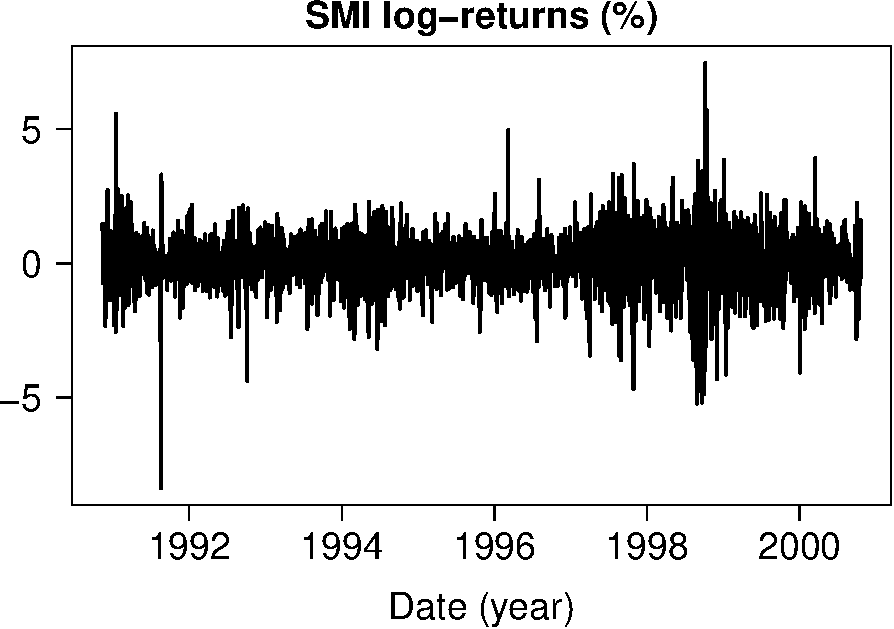
\includegraphics{MS-GARCH_files/figure-latex/unnamed-chunk-9-1.pdf}

\begin{Shaded}
\begin{Highlighting}[]
\CommentTok{\#dev.off()}
\end{Highlighting}
\end{Shaded}

\begin{Shaded}
\begin{Highlighting}[]
\DocumentationTok{\#\#\#\#\#\#\#\#\#\#\#\#\#\#\#\#\#\#\#\#\#\#}
\DocumentationTok{\#\#     FIGURE 2     \#\#}
\DocumentationTok{\#\#\#\#\#\#\#\#\#\#\#\#\#\#\#\#\#\#\#\#\#\#}

\CommentTok{\#pdf(file = "figure2.pdf", height = 13, width = 16, compress = TRUE)}
\NormalTok{op }\OtherTok{\textless{}{-}} \FunctionTok{par}\NormalTok{(}\AttributeTok{mfrow =} \FunctionTok{c}\NormalTok{(}\DecValTok{2}\NormalTok{,}\DecValTok{1}\NormalTok{),}
          \AttributeTok{oma =} \FunctionTok{c}\NormalTok{(}\DecValTok{1}\NormalTok{,}\DecValTok{1}\NormalTok{,}\DecValTok{0}\NormalTok{,}\DecValTok{0}\NormalTok{) }\SpecialCharTok{+} \FloatTok{0.0}\NormalTok{,}
          \AttributeTok{mar =} \FunctionTok{c}\NormalTok{(}\DecValTok{2}\NormalTok{,}\DecValTok{2}\NormalTok{,}\DecValTok{2}\NormalTok{,}\DecValTok{2}\NormalTok{) }\SpecialCharTok{+} \FloatTok{0.0}\NormalTok{)}
\FunctionTok{plot}\NormalTok{(}\FunctionTok{as.vector}\NormalTok{(SMI), }\AttributeTok{las =} \DecValTok{1}\NormalTok{, }\AttributeTok{type =} \StringTok{\textquotesingle{}p\textquotesingle{}}\NormalTok{, }\AttributeTok{pch =} \DecValTok{20}\NormalTok{, }\AttributeTok{col =} \StringTok{\textquotesingle{}black\textquotesingle{}}\NormalTok{,}
     \AttributeTok{cex =} \FloatTok{1.5}\NormalTok{, }\AttributeTok{axes =} \ConstantTok{FALSE}\NormalTok{, }\AttributeTok{ann =} \ConstantTok{FALSE}\NormalTok{)}
\FunctionTok{par}\NormalTok{(}\AttributeTok{new =} \ConstantTok{TRUE}\NormalTok{)}
\NormalTok{ylabel }\OtherTok{\textless{}{-}} \FunctionTok{expression}\NormalTok{(}\FunctionTok{paste}\NormalTok{(}\StringTok{"Pr("}\NormalTok{, s[t], }\StringTok{" = 2 | "}\NormalTok{, }\FunctionTok{hat}\NormalTok{(psi), }\StringTok{", "}\NormalTok{, I[t], }\StringTok{")"}\NormalTok{))}
\FunctionTok{plot}\NormalTok{(zoo}\SpecialCharTok{::}\FunctionTok{zoo}\NormalTok{(smoothed.prob, }\AttributeTok{order.by =}\NormalTok{ zoo}\SpecialCharTok{::}\FunctionTok{index}\NormalTok{(SMI)), }\AttributeTok{lty =} \DecValTok{1}\NormalTok{, }\AttributeTok{plot.type =} \StringTok{"single"}\NormalTok{,}
     \AttributeTok{col =} \StringTok{"red"}\NormalTok{, }\AttributeTok{las =} \DecValTok{1}\NormalTok{, }\AttributeTok{ylab =} \StringTok{""}\NormalTok{, }\AttributeTok{xlab =} \StringTok{"Date"}\NormalTok{, }\AttributeTok{lwd =} \DecValTok{3}\NormalTok{, }\AttributeTok{cex.axis =} \FloatTok{1.5}\NormalTok{, }\AttributeTok{cex.lab =} \FloatTok{1.5}\NormalTok{)}
\FunctionTok{title}\NormalTok{(}\AttributeTok{main =} \StringTok{"Smoothed probabilities"}\NormalTok{, }\AttributeTok{cex.main =} \FloatTok{1.5}\NormalTok{)}
\FunctionTok{plot}\NormalTok{(zoo}\SpecialCharTok{::}\FunctionTok{zoo}\NormalTok{(vol, }\AttributeTok{order.by =}\NormalTok{ zoo}\SpecialCharTok{::}\FunctionTok{index}\NormalTok{(SMI)), }\AttributeTok{lty =} \DecValTok{1}\NormalTok{, }\AttributeTok{plot.type =} \StringTok{"single"}\NormalTok{,}
     \AttributeTok{col =} \StringTok{"black"}\NormalTok{, }\AttributeTok{las =} \DecValTok{1}\NormalTok{, }\AttributeTok{ylab =} \StringTok{""}\NormalTok{, }\AttributeTok{xlab =} \StringTok{"Date"}\NormalTok{, }\AttributeTok{lwd =} \DecValTok{3}\NormalTok{, }\AttributeTok{cex.axis =} \FloatTok{1.5}\NormalTok{, }\AttributeTok{cex.lab =} \FloatTok{1.5}\NormalTok{)}
\FunctionTok{title}\NormalTok{(}\AttributeTok{main =} \StringTok{"Volatility (\%)"}\NormalTok{, }\AttributeTok{cex.main =} \FloatTok{1.5}\NormalTok{)}
\end{Highlighting}
\end{Shaded}

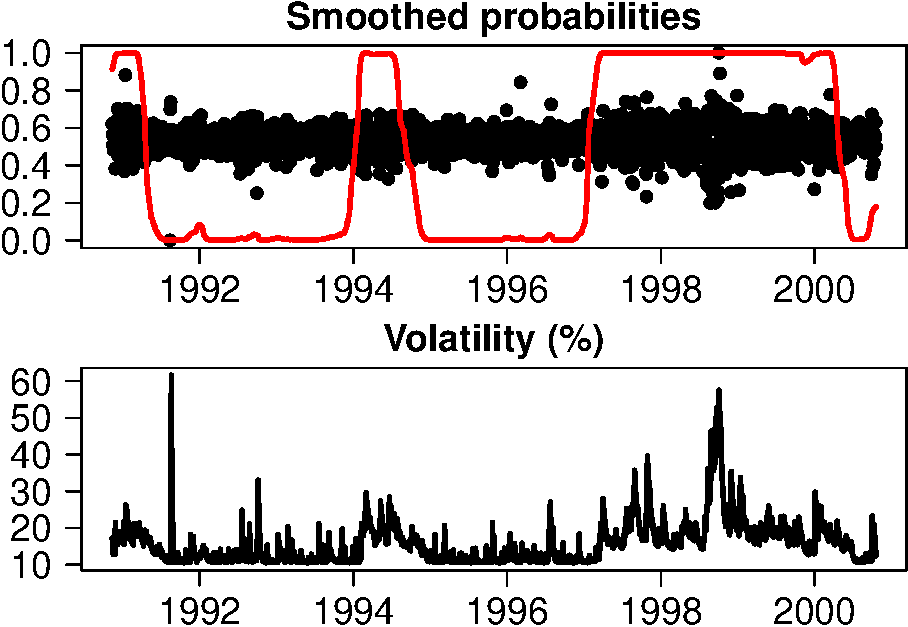
\includegraphics{MS-GARCH_files/figure-latex/unnamed-chunk-10-1.pdf}

\begin{Shaded}
\begin{Highlighting}[]
\FunctionTok{par}\NormalTok{(op)}
\CommentTok{\#dev.off()}
\end{Highlighting}
\end{Shaded}

\begin{Shaded}
\begin{Highlighting}[]
\DocumentationTok{\#\#\#\#\#\#\#\#\#\#\#\#\#\#\#\#\#\#\#\#\#\#}
\DocumentationTok{\#\#     FIGURE 3     \#\#}
\DocumentationTok{\#\#\#\#\#\#\#\#\#\#\#\#\#\#\#\#\#\#\#\#\#\#}

\NormalTok{sel }\OtherTok{\textless{}{-}} \FunctionTok{c}\NormalTok{(}\StringTok{"alpha1\_1"}\NormalTok{, }\StringTok{"alpha2\_1"}\NormalTok{)}
\NormalTok{tmp }\OtherTok{\textless{}{-}}\NormalTok{ draws[, sel]}
\NormalTok{par.mle }\OtherTok{\textless{}{-}}\NormalTok{ fit.ml}\SpecialCharTok{$}\NormalTok{par[sel]}
\NormalTok{par.bay }\OtherTok{\textless{}{-}} \FunctionTok{apply}\NormalTok{(tmp, }\DecValTok{2}\NormalTok{, mean)}
\NormalTok{xlim }\OtherTok{\textless{}{-}} \FunctionTok{range}\NormalTok{(}\FunctionTok{c}\NormalTok{(tmp[,}\DecValTok{1}\NormalTok{], par.mle[}\DecValTok{1}\NormalTok{]))}
\NormalTok{ylim }\OtherTok{\textless{}{-}} \FunctionTok{range}\NormalTok{(}\FunctionTok{c}\NormalTok{(tmp[,}\DecValTok{2}\NormalTok{], par.mle[}\DecValTok{2}\NormalTok{]))}
\CommentTok{\#pdf(file = "figure3.pdf", height = 13, width = 13, compress = TRUE)}
\FunctionTok{par}\NormalTok{(}\AttributeTok{mfrow =} \FunctionTok{c}\NormalTok{(}\DecValTok{1}\NormalTok{, }\DecValTok{1}\NormalTok{))}
\FunctionTok{plot}\NormalTok{(tmp, }\AttributeTok{pch =} \DecValTok{20}\NormalTok{, }\AttributeTok{las =} \DecValTok{1}\NormalTok{, }\AttributeTok{lwd =} \DecValTok{2}\NormalTok{, }\AttributeTok{cex =} \DecValTok{2}\NormalTok{, }\AttributeTok{xlim =}\NormalTok{ xlim, }\AttributeTok{ylim =}\NormalTok{ ylim,}
     \AttributeTok{col =} \StringTok{"lightsteelblue"}\NormalTok{, }\AttributeTok{cex.axis =} \FloatTok{1.5}\NormalTok{, }\AttributeTok{cex.lab =} \FloatTok{1.5}\NormalTok{)}
\FunctionTok{grid}\NormalTok{()}
\FunctionTok{par}\NormalTok{(}\AttributeTok{new =} \ConstantTok{TRUE}\NormalTok{)}
\FunctionTok{points}\NormalTok{(par.bay[}\DecValTok{1}\NormalTok{], par.bay[}\DecValTok{2}\NormalTok{], }\AttributeTok{cex =} \DecValTok{4}\NormalTok{, }\AttributeTok{lwd =} \DecValTok{2}\NormalTok{,}
       \AttributeTok{pch =} \DecValTok{15}\NormalTok{, }\AttributeTok{col =} \StringTok{"blue"}\NormalTok{, }\AttributeTok{xlim =}\NormalTok{ xlim, }\AttributeTok{ylim =}\NormalTok{ ylim)}
\FunctionTok{points}\NormalTok{(par.mle[}\DecValTok{1}\NormalTok{], par.mle[}\DecValTok{2}\NormalTok{], }\AttributeTok{cex =} \DecValTok{4}\NormalTok{, }\AttributeTok{lwd =} \DecValTok{2}\NormalTok{,}
       \AttributeTok{pch =} \DecValTok{17}\NormalTok{, }\AttributeTok{col =} \StringTok{"red"}\NormalTok{, }\AttributeTok{xlim =}\NormalTok{ xlim, }\AttributeTok{ylim =}\NormalTok{ ylim)}
\end{Highlighting}
\end{Shaded}

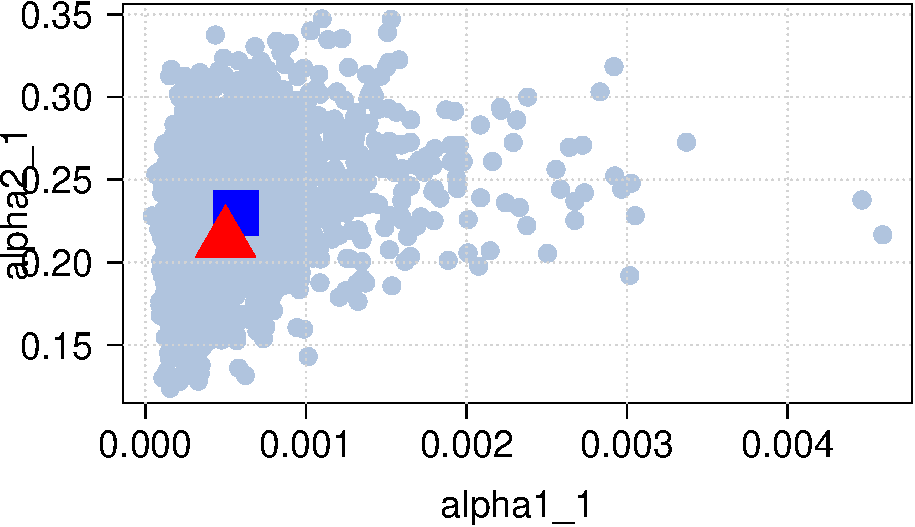
\includegraphics{MS-GARCH_files/figure-latex/unnamed-chunk-11-1.pdf}

\begin{Shaded}
\begin{Highlighting}[]
\CommentTok{\#dev.off()}
\end{Highlighting}
\end{Shaded}

\begin{Shaded}
\begin{Highlighting}[]
\DocumentationTok{\#\#\#\#\#\#\#\#\#\#\#\#\#\#\#\#\#\#\#\#\#\#}
\DocumentationTok{\#\#     FIGURE 4     \#\#}
\DocumentationTok{\#\#\#\#\#\#\#\#\#\#\#\#\#\#\#\#\#\#\#\#\#\#}

\NormalTok{n }\OtherTok{\textless{}{-}} \FunctionTok{length}\NormalTok{(ucvol.draws}\SpecialCharTok{$}\NormalTok{ucvol\_1)}
\CommentTok{\#pdf(file = "figure4.pdf", height = 13, width = 16, compress = TRUE)}
\NormalTok{op }\OtherTok{\textless{}{-}} \FunctionTok{par}\NormalTok{(}\AttributeTok{mar =} \FunctionTok{c}\NormalTok{(}\DecValTok{2}\NormalTok{, }\DecValTok{2}\NormalTok{, }\DecValTok{2}\NormalTok{, }\DecValTok{2}\NormalTok{),}
          \AttributeTok{mfrow =} \FunctionTok{c}\NormalTok{(}\DecValTok{1}\NormalTok{, }\DecValTok{2}\NormalTok{),}
          \AttributeTok{oma =} \FunctionTok{c}\NormalTok{(}\DecValTok{2}\NormalTok{, }\DecValTok{2}\NormalTok{, }\FloatTok{0.2}\NormalTok{, }\FloatTok{0.2}\NormalTok{))}
\FunctionTok{hist}\NormalTok{(ucvol.draws}\SpecialCharTok{$}\NormalTok{ucvol\_1, }\AttributeTok{nclass =} \FunctionTok{round}\NormalTok{(}\DecValTok{10} \SpecialCharTok{*} \FunctionTok{log}\NormalTok{(n)), }\AttributeTok{prob =} \ConstantTok{TRUE}\NormalTok{,}
     \AttributeTok{col =} \StringTok{"lightsteelblue"}\NormalTok{, }\AttributeTok{las =} \DecValTok{1}\NormalTok{, }\AttributeTok{xlab =} \StringTok{"Volatility (\%)"}\NormalTok{,}
     \AttributeTok{ylab =} \StringTok{""}\NormalTok{, }\AttributeTok{cex.lab =} \FloatTok{1.5}\NormalTok{, }\AttributeTok{cex.axis =} \FloatTok{1.5}\NormalTok{, }\AttributeTok{main =} \StringTok{""}\NormalTok{)}
\FunctionTok{title}\NormalTok{(}\AttributeTok{main =} \StringTok{"Regime 1"}\NormalTok{, }\AttributeTok{cex.main =} \FloatTok{1.5}\NormalTok{)}
\FunctionTok{lines}\NormalTok{(}\FunctionTok{density}\NormalTok{(ucvol.draws}\SpecialCharTok{$}\NormalTok{ucvol\_1), }\AttributeTok{col =} \StringTok{"black"}\NormalTok{, }\AttributeTok{lwd =} \DecValTok{2}\NormalTok{)}
\FunctionTok{rug}\NormalTok{(ucvol.draws}\SpecialCharTok{$}\NormalTok{ucvol\_1); }\FunctionTok{box}\NormalTok{()}
\FunctionTok{points}\NormalTok{(ucvol.bay}\SpecialCharTok{$}\NormalTok{ucvol\_1, }\DecValTok{0}\NormalTok{, }\AttributeTok{pch =} \DecValTok{15}\NormalTok{, }\AttributeTok{col =} \StringTok{"blue"}\NormalTok{, }\AttributeTok{lwd =} \DecValTok{2}\NormalTok{, }\AttributeTok{cex =} \DecValTok{3}\NormalTok{)}
\FunctionTok{points}\NormalTok{(ucvol.mle}\SpecialCharTok{$}\NormalTok{ucvol\_1, }\DecValTok{0}\NormalTok{, }\AttributeTok{pch =} \DecValTok{17}\NormalTok{, }\AttributeTok{col =} \StringTok{"red"}\NormalTok{, }\AttributeTok{lwd =} \DecValTok{2}\NormalTok{, }\AttributeTok{cex =} \DecValTok{3}\NormalTok{)}
\FunctionTok{hist}\NormalTok{(ucvol.draws}\SpecialCharTok{$}\NormalTok{ucvol\_2, }\AttributeTok{nclass =} \FunctionTok{round}\NormalTok{(}\DecValTok{10} \SpecialCharTok{*} \FunctionTok{log}\NormalTok{(n)), }\AttributeTok{prob =} \ConstantTok{TRUE}\NormalTok{,}
     \AttributeTok{col =} \StringTok{"lightsteelblue"}\NormalTok{, }\AttributeTok{las =} \DecValTok{1}\NormalTok{, }\AttributeTok{xlab =} \StringTok{"Volatility (\%)"}\NormalTok{,}
     \AttributeTok{ylab =} \StringTok{""}\NormalTok{, }\AttributeTok{cex.lab =} \FloatTok{1.5}\NormalTok{, }\AttributeTok{cex.axis =} \FloatTok{1.5}\NormalTok{, }\AttributeTok{main =} \StringTok{""}\NormalTok{)}
\FunctionTok{rug}\NormalTok{(ucvol.draws}\SpecialCharTok{$}\NormalTok{ucvol\_2); }\FunctionTok{box}\NormalTok{()}
\FunctionTok{points}\NormalTok{(ucvol.bay}\SpecialCharTok{$}\NormalTok{ucvol\_2, }\DecValTok{0}\NormalTok{, }\AttributeTok{pch =} \DecValTok{15}\NormalTok{, }\AttributeTok{col =} \StringTok{"blue"}\NormalTok{, }\AttributeTok{lwd =} \DecValTok{2}\NormalTok{, }\AttributeTok{cex =} \DecValTok{3}\NormalTok{)}
\FunctionTok{points}\NormalTok{(ucvol.mle}\SpecialCharTok{$}\NormalTok{ucvol\_2, }\DecValTok{0}\NormalTok{, }\AttributeTok{pch =} \DecValTok{17}\NormalTok{, }\AttributeTok{col =} \StringTok{"red"}\NormalTok{, }\AttributeTok{lwd =} \DecValTok{2}\NormalTok{, }\AttributeTok{cex =} \DecValTok{3}\NormalTok{)}
\FunctionTok{title}\NormalTok{(}\AttributeTok{main =} \StringTok{"Regime 2"}\NormalTok{, }\AttributeTok{cex.main =} \FloatTok{1.5}\NormalTok{)}
\FunctionTok{lines}\NormalTok{(}\FunctionTok{density}\NormalTok{(ucvol.draws}\SpecialCharTok{$}\NormalTok{ucvol\_2), }\AttributeTok{col =} \StringTok{"black"}\NormalTok{, }\AttributeTok{lwd =} \DecValTok{2}\NormalTok{)}
\end{Highlighting}
\end{Shaded}

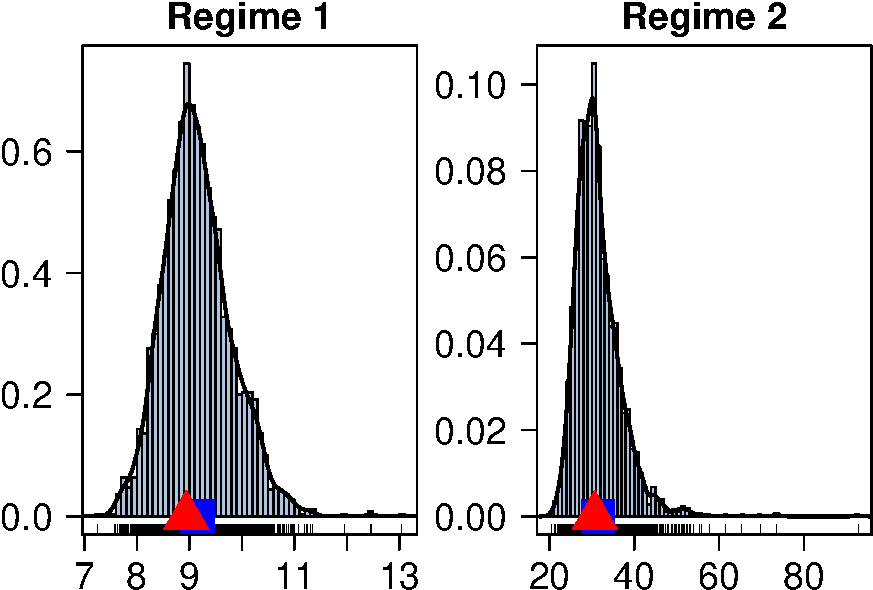
\includegraphics{MS-GARCH_files/figure-latex/unnamed-chunk-12-1.pdf}

\begin{Shaded}
\begin{Highlighting}[]
\FunctionTok{par}\NormalTok{(op)}
\CommentTok{\#dev.off()}
\end{Highlighting}
\end{Shaded}

\begin{Shaded}
\begin{Highlighting}[]
\DocumentationTok{\#\#\#\#\#\#\#\#\#\#\#\#\#\#\#\#\#\#\#\#\#\#}
\DocumentationTok{\#\#     FIGURE 5     \#\#}
\DocumentationTok{\#\#\#\#\#\#\#\#\#\#\#\#\#\#\#\#\#\#\#\#\#\#}

\CommentTok{\#pdf(file = "figure5.pdf", height = 13, width = 16, compress = TRUE)}
\CommentTok{\#png(filename = "figure5.png", height = 13, width = 16, units = "in", res = 600)}
\NormalTok{xlim }\OtherTok{\textless{}{-}} \FunctionTok{c}\NormalTok{(}\SpecialCharTok{{-}}\DecValTok{4}\NormalTok{, }\SpecialCharTok{{-}}\FloatTok{1.2}\NormalTok{)}
\NormalTok{ylim }\OtherTok{\textless{}{-}} \FunctionTok{c}\NormalTok{(}\DecValTok{0}\NormalTok{, }\FloatTok{0.1}\NormalTok{)}
\FunctionTok{par}\NormalTok{(}\AttributeTok{mfrow =} \FunctionTok{c}\NormalTok{(}\DecValTok{1}\NormalTok{, }\DecValTok{1}\NormalTok{))}
\FunctionTok{matplot}\NormalTok{(x, }\FunctionTok{t}\NormalTok{(pred.draws), }\AttributeTok{xlim =}\NormalTok{ xlim, }\AttributeTok{ylim =}\NormalTok{ ylim,}
        \AttributeTok{type =} \StringTok{"l"}\NormalTok{, }\AttributeTok{col =} \StringTok{"lightsteelblue"}\NormalTok{,}
        \AttributeTok{xlab =} \StringTok{"Return (\%)"}\NormalTok{, }\AttributeTok{ylab =} \StringTok{"Predictives"}\NormalTok{,}
        \AttributeTok{lty =} \FloatTok{1.5}\NormalTok{, }\AttributeTok{las =} \DecValTok{1}\NormalTok{, }\AttributeTok{cex.axis =} \FloatTok{1.5}\NormalTok{, }\AttributeTok{cex.lab =} \FloatTok{1.5}\NormalTok{)}
\FunctionTok{title}\NormalTok{(}\AttributeTok{main =} \StringTok{"Left{-}tail forecast of SMI index return"}\NormalTok{, }\AttributeTok{cex.main =} \FloatTok{1.5}\NormalTok{)}
\FunctionTok{lines}\NormalTok{(x, pred.bay, }\AttributeTok{xlim =}\NormalTok{ xlim, }\AttributeTok{ylim =}\NormalTok{ ylim,}
      \AttributeTok{type =} \StringTok{"l"}\NormalTok{, }\AttributeTok{lty =} \StringTok{"solid"}\NormalTok{, }\AttributeTok{col =} \StringTok{"blue"}\NormalTok{, }\AttributeTok{lwd =} \DecValTok{3}\NormalTok{)}
\FunctionTok{lines}\NormalTok{(x, pred.mle, }\AttributeTok{xlim =}\NormalTok{ xlim, }\AttributeTok{ylim =}\NormalTok{ ylim,}
      \AttributeTok{type =} \StringTok{"l"}\NormalTok{, }\AttributeTok{pch =} \StringTok{"o"}\NormalTok{, }\AttributeTok{lty =} \StringTok{"dashed"}\NormalTok{, }\AttributeTok{col =} \StringTok{"red"}\NormalTok{, }\AttributeTok{lwd =} \DecValTok{3}\NormalTok{)}
\FunctionTok{legend}\NormalTok{(}\StringTok{"topleft"}\NormalTok{, }\FunctionTok{c}\NormalTok{(}\StringTok{"MCMC draws"}\NormalTok{, }\StringTok{"Bayesian"}\NormalTok{,}\StringTok{"ML"}\NormalTok{),}
       \AttributeTok{col =} \FunctionTok{c}\NormalTok{(}\StringTok{"lightsteelblue"}\NormalTok{, }\StringTok{"blue"}\NormalTok{, }\StringTok{"red"}\NormalTok{), }\AttributeTok{lwd =} \DecValTok{3}\NormalTok{,}
       \AttributeTok{lty =} \FunctionTok{c}\NormalTok{(}\DecValTok{1}\NormalTok{, }\DecValTok{1}\NormalTok{, }\DecValTok{2}\NormalTok{), }\AttributeTok{bty =} \StringTok{"n"}\NormalTok{, }\AttributeTok{cex =} \DecValTok{2}\NormalTok{)}
\FunctionTok{box}\NormalTok{()}
\end{Highlighting}
\end{Shaded}

\includegraphics{MS-GARCH_files/figure-latex/unnamed-chunk-13-1.pdf}

\begin{Shaded}
\begin{Highlighting}[]
\CommentTok{\#dev.off()}
\end{Highlighting}
\end{Shaded}

\begin{Shaded}
\begin{Highlighting}[]
\DocumentationTok{\#\#\#\#\#\#\#\#\#\#\#\#\#\#\#\#\#\#\#\#\#\#}
\DocumentationTok{\#\#     FIGURE 6     \#\#}
\DocumentationTok{\#\#\#\#\#\#\#\#\#\#\#\#\#\#\#\#\#\#\#\#\#\#}

\FunctionTok{library}\NormalTok{(}\StringTok{"zoo"}\NormalTok{)}
\end{Highlighting}
\end{Shaded}

\begin{verbatim}
## 
## Attaching package: 'zoo'
\end{verbatim}

\begin{verbatim}
## The following objects are masked from 'package:base':
## 
##     as.Date, as.Date.numeric
\end{verbatim}

\begin{Shaded}
\begin{Highlighting}[]
\NormalTok{time.index }\OtherTok{\textless{}{-}}\NormalTok{ zoo}\SpecialCharTok{::}\FunctionTok{index}\NormalTok{(SMI)[(n.its }\SpecialCharTok{+} \DecValTok{1}\NormalTok{)}\SpecialCharTok{:}\NormalTok{(n.ots }\SpecialCharTok{+}\NormalTok{ n.its)]}
\NormalTok{y\_ots }\OtherTok{\textless{}{-}}\NormalTok{ zoo}\SpecialCharTok{::}\FunctionTok{zoo}\NormalTok{(y.ots, }\AttributeTok{order.by =}\NormalTok{ time.index)}
\NormalTok{VaR   }\OtherTok{\textless{}{-}}\NormalTok{ zoo}\SpecialCharTok{::}\FunctionTok{zoo}\NormalTok{(VaR, }\AttributeTok{order.by =}\NormalTok{ time.index)}

\DocumentationTok{\#\# pdf(file = "figure6.pdf", height = 13, width = 16, compress = TRUE)}
\FunctionTok{par}\NormalTok{(}\AttributeTok{mfrow =} \FunctionTok{c}\NormalTok{(}\DecValTok{1}\NormalTok{, }\DecValTok{1}\NormalTok{))}
\FunctionTok{plot}\NormalTok{(y\_ots, }\AttributeTok{type =} \StringTok{\textquotesingle{}p\textquotesingle{}}\NormalTok{, }\AttributeTok{las =} \DecValTok{1}\NormalTok{, }\AttributeTok{lwd =} \DecValTok{1}\NormalTok{, }\AttributeTok{xlab =} \StringTok{"Date (year)"}\NormalTok{,}
     \AttributeTok{ylab =} \StringTok{""}\NormalTok{, }\AttributeTok{col =} \StringTok{"black"}\NormalTok{, }\AttributeTok{cex.axis =} \FloatTok{1.5}\NormalTok{, }\AttributeTok{cex.lab =} \FloatTok{1.5}\NormalTok{, }\AttributeTok{pch =} \DecValTok{19}\NormalTok{)}
\FunctionTok{lines}\NormalTok{(VaR[,}\DecValTok{1}\NormalTok{], }\AttributeTok{type =} \StringTok{\textquotesingle{}l\textquotesingle{}}\NormalTok{, }\AttributeTok{col =} \StringTok{"red"}\NormalTok{, }\AttributeTok{lwd =} \DecValTok{3}\NormalTok{, }\AttributeTok{lty =} \StringTok{"dashed"}\NormalTok{)}
\FunctionTok{lines}\NormalTok{(VaR[,}\DecValTok{2}\NormalTok{], }\AttributeTok{type =} \StringTok{\textquotesingle{}l\textquotesingle{}}\NormalTok{, }\AttributeTok{col =} \StringTok{"blue"}\NormalTok{, }\AttributeTok{lwd =} \DecValTok{3}\NormalTok{)}
\FunctionTok{legend}\NormalTok{(}\StringTok{"topleft"}\NormalTok{, }\AttributeTok{legend =} \FunctionTok{c}\NormalTok{(}\StringTok{"VaR 5\% {-} GJR{-}std"}\NormalTok{, }\StringTok{"VaR 5\% {-} MS2{-}GJR{-}std"}\NormalTok{),}
       \AttributeTok{col =} \FunctionTok{c}\NormalTok{(}\StringTok{"red"}\NormalTok{, }\StringTok{"blue"}\NormalTok{), }\AttributeTok{lwd =} \DecValTok{3}\NormalTok{, }\AttributeTok{cex =} \FloatTok{1.5}\NormalTok{, }\AttributeTok{lty =} \FunctionTok{c}\NormalTok{(}\StringTok{"dashed"}\NormalTok{, }\StringTok{"solid"}\NormalTok{))}
\FunctionTok{abline}\NormalTok{(}\AttributeTok{h =} \DecValTok{0}\NormalTok{)}
\FunctionTok{title}\NormalTok{(}\StringTok{"Backtesing VaR at 5\% risk level"}\NormalTok{, }\AttributeTok{cex.main =} \FloatTok{1.5}\NormalTok{)}
\end{Highlighting}
\end{Shaded}

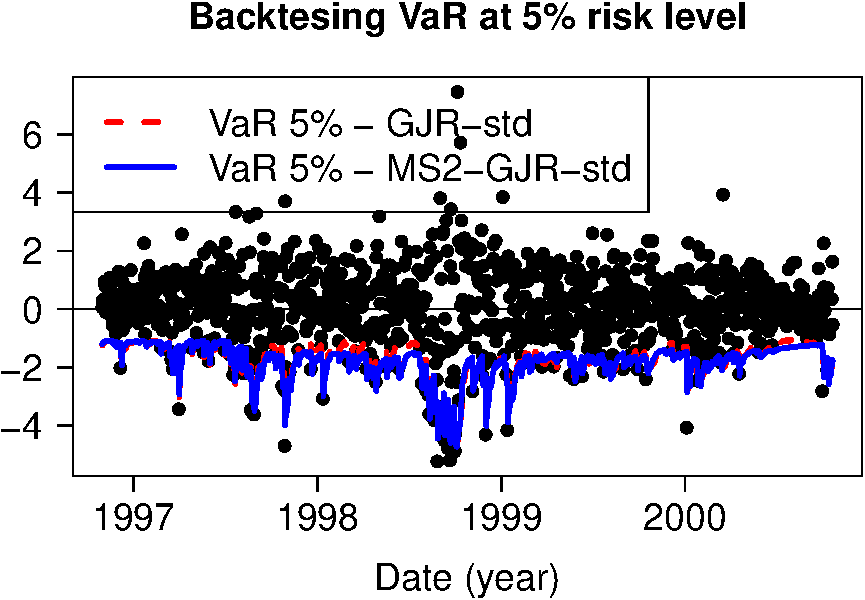
\includegraphics{MS-GARCH_files/figure-latex/unnamed-chunk-14-1.pdf}

\begin{Shaded}
\begin{Highlighting}[]
\CommentTok{\#dev.off()}
\end{Highlighting}
\end{Shaded}


\end{document}
